\documentclass[a4paper,11pt]{article}%,twocolumn
%% packages


\usepackage{amsmath} % needed for command eqref
\usepackage{amssymb} % needed for math fonts
\usepackage[colorlinks=true,breaklinks]{hyperref} % needed for creating hyperlinks in the document, the option colorlinks=true gets rid of the awful boxes, breaklinks breaks lonkg links (list of figures), and ngerman sets everything for german as default hyperlinks language
\usepackage[hyphenbreaks]{breakurl} % ben�tigt f�r das Brechen von URLs in Literaturreferenzen, hyphenbreaks auch bei links, die �ber eine Seite gehen (mit hyphenation).
\usepackage{xcolor}
\definecolor{c1}{rgb}{0,0,1} % blue
\definecolor{c2}{rgb}{0,0.3,0.9} % light blue
\definecolor{c3}{rgb}{0.3,0,0.9} % red blue
\hypersetup{
    linkcolor={c1}, % internal links
    citecolor={c2}, % citations
    urlcolor={c3} % external links/urls
}
%\usepackage{cite} % needed for cite
\usepackage[square,authoryear]{natbib} % needed for cite and abbrvnat bibliography style
\usepackage[nottoc]{tocbibind} % needed for displaying bibliography and other in the table of contents
\usepackage{graphicx} % needed for \includegraphics 
\usepackage{longtable} % needed for long tables over pages
\usepackage{bigstrut} % needed for the command \bigstrut
\usepackage{enumerate} % needed for some options in enumerate
%\usepackage{todonotes} % needed for todos
\usepackage{makeidx} % needed for creating an index
\makeindex
\usepackage{gensymb}
\usepackage{url}
\usepackage{psfrag}
\usepackage{multirow}
\usepackage{subfigure}
\usepackage{epstopdf}

%% page settings
\usepackage[top=10mm, bottom=15mm,left=10mm,right=10mm]{geometry}  
 % needed for page border settings
\parindent=0mm % for space of first line of new text block

\sloppy % for writing with hyphenless justification (tries to)
\hyphenation{} % use hyphenation of tolerance parametershttp://www.jr-x.de/publikationen/latex/tipps/zeilenumbruch.html
\hyphenpenalty=10000
\exhyphenpenalty=10000
\usepackage{fancyhdr} % needed for head and foot options
    \usepackage[breakable]{tcolorbox}
    \usepackage{xcolor} % Allow colors to be defined  
    \usepackage{textcomp} % defines textquotesingle
    \usepackage{upquote} % Upright quotes for verbatim code
    \usepackage{eurosym} % defines \euro
    \usepackage[mathletters]{ucs} % Extended unicode (utf-8) support
    \usepackage{fancyvrb} % verbatim replacement that allows latex
    \usepackage{grffile} % extends the file name processing of package graphics 
                         % to support a larger range
    \makeatletter % fix for old versions of grffile with XeLaTeX
    \@ifpackagelater{grffile}{2019/11/01}
    {
      % Do nothing on new versions
    }
    {
      \def\Gread@@xetex#1{%
        \IfFileExists{"\Gin@base".bb}%
        {\Gread@eps{\Gin@base.bb}}%
        {\Gread@@xetex@aux#1}%
      }
    }
    \makeatother
    \usepackage{titling}
    \usepackage{longtable} % longtable support required by pandoc >1.10
    \usepackage{booktabs}  % table support for pandoc > 1.12.2
    \usepackage[inline]{enumitem} % IRkernel/repr support (it uses the enumerate* environment)
    \usepackage[normalem]{ulem} % ulem is needed to support strikethroughs (\sout)
                                % normalem makes italics be italics, not underlines
    \usepackage{mathrsfs}
    

    % ANSI colors
    \definecolor{ansi-black}{HTML}{3E424D}
    \definecolor{ansi-black-intense}{HTML}{282C36}
    \definecolor{ansi-red}{HTML}{E75C58}
    \definecolor{ansi-red-intense}{HTML}{B22B31}
    \definecolor{ansi-green}{HTML}{00A250}
    \definecolor{ansi-green-intense}{HTML}{007427}
    \definecolor{ansi-yellow}{HTML}{DDB62B}
    \definecolor{ansi-yellow-intense}{HTML}{B27D12}
    \definecolor{ansi-blue}{HTML}{208FFB}
    \definecolor{ansi-blue-intense}{HTML}{0065CA}
    \definecolor{ansi-magenta}{HTML}{D160C4}
    \definecolor{ansi-magenta-intense}{HTML}{A03196}
    \definecolor{ansi-cyan}{HTML}{60C6C8}
    \definecolor{ansi-cyan-intense}{HTML}{258F8F}
    \definecolor{ansi-white}{HTML}{C5C1B4}
    \definecolor{ansi-white-intense}{HTML}{A1A6B2}
    \definecolor{ansi-default-inverse-fg}{HTML}{FFFFFF}
    \definecolor{ansi-default-inverse-bg}{HTML}{000000}

    % common color for the border for error outputs.
    \definecolor{outerrorbackground}{HTML}{FFDFDF}

    % commands and environments needed by pandoc snippets
    % extracted from the output of `pandoc -s`
    \providecommand{\tightlist}{%
      \setlength{\itemsep}{0pt}\setlength{\parskip}{0pt}}
    \DefineVerbatimEnvironment{Highlighting}{Verbatim}{commandchars=\\\{\}}
    %' for more characters per line
    \newenvironment{Shaded}{}{}
    \newcommand{\KeywordTok}[1]{\textcolor[rgb]{0.00,0.44,0.13}{\textbf{{#1}}}}
    \newcommand{\DataTypeTok}[1]{\textcolor[rgb]{0.56,0.13,0.00}{{#1}}}
    \newcommand{\DecValTok}[1]{\textcolor[rgb]{0.25,0.63,0.44}{{#1}}}
    \newcommand{\BaseNTok}[1]{\textcolor[rgb]{0.25,0.63,0.44}{{#1}}}
    \newcommand{\FloatTok}[1]{\textcolor[rgb]{0.25,0.63,0.44}{{#1}}}
    \newcommand{\CharTok}[1]{\textcolor[rgb]{0.25,0.44,0.63}{{#1}}}
    \newcommand{\StringTok}[1]{\textcolor[rgb]{0.25,0.44,0.63}{{#1}}}
    \newcommand{\CommentTok}[1]{\textcolor[rgb]{0.38,0.63,0.69}{\textit{{#1}}}}
    \newcommand{\OtherTok}[1]{\textcolor[rgb]{0.00,0.44,0.13}{{#1}}}
    \newcommand{\AlertTok}[1]{\textcolor[rgb]{1.00,0.00,0.00}{\textbf{{#1}}}}
    \newcommand{\FunctionTok}[1]{\textcolor[rgb]{0.02,0.16,0.49}{{#1}}}
    \newcommand{\RegionMarkerTok}[1]{{#1}}
    \newcommand{\ErrorTok}[1]{\textcolor[rgb]{1.00,0.00,0.00}{\textbf{{#1}}}}
    \newcommand{\NormalTok}[1]{{#1}}
    
    % Additional commands for more recent versions of Pandoc
    \newcommand{\ConstantTok}[1]{\textcolor[rgb]{0.53,0.00,0.00}{{#1}}}
    \newcommand{\SpecialCharTok}[1]{\textcolor[rgb]{0.25,0.44,0.63}{{#1}}}
    \newcommand{\VerbatimStringTok}[1]{\textcolor[rgb]{0.25,0.44,0.63}{{#1}}}
    \newcommand{\SpecialStringTok}[1]{\textcolor[rgb]{0.73,0.40,0.53}{{#1}}}
    \newcommand{\ImportTok}[1]{{#1}}
    \newcommand{\DocumentationTok}[1]{\textcolor[rgb]{0.73,0.13,0.13}{\textit{{#1}}}}
    \newcommand{\AnnotationTok}[1]{\textcolor[rgb]{0.38,0.63,0.69}{\textbf{\textit{{#1}}}}}
    \newcommand{\CommentVarTok}[1]{\textcolor[rgb]{0.38,0.63,0.69}{\textbf{\textit{{#1}}}}}
    \newcommand{\VariableTok}[1]{\textcolor[rgb]{0.10,0.09,0.49}{{#1}}}
    \newcommand{\ControlFlowTok}[1]{\textcolor[rgb]{0.00,0.44,0.13}{\textbf{{#1}}}}
    \newcommand{\OperatorTok}[1]{\textcolor[rgb]{0.40,0.40,0.40}{{#1}}}
    \newcommand{\BuiltInTok}[1]{{#1}}
    \newcommand{\ExtensionTok}[1]{{#1}}
    \newcommand{\PreprocessorTok}[1]{\textcolor[rgb]{0.74,0.48,0.00}{{#1}}}
    \newcommand{\AttributeTok}[1]{\textcolor[rgb]{0.49,0.56,0.16}{{#1}}}
    \newcommand{\InformationTok}[1]{\textcolor[rgb]{0.38,0.63,0.69}{\textbf{\textit{{#1}}}}}
    \newcommand{\WarningTok}[1]{\textcolor[rgb]{0.38,0.63,0.69}{\textbf{\textit{{#1}}}}}
    
    
    % Define a nice break command that doesn't care if a line doesn't already
    % exist.
    \def\br{\hspace*{\fill} \\* }

% Pygments definitions
\makeatletter
\def\PY@reset{\let\PY@it=\relax \let\PY@bf=\relax%
    \let\PY@ul=\relax \let\PY@tc=\relax%
    \let\PY@bc=\relax \let\PY@ff=\relax}
\def\PY@tok#1{\csname PY@tok@#1\endcsname}
\def\PY@toks#1+{\ifx\relax#1\empty\else%
    \PY@tok{#1}\expandafter\PY@toks\fi}
\def\PY@do#1{\PY@bc{\PY@tc{\PY@ul{%
    \PY@it{\PY@bf{\PY@ff{#1}}}}}}}
\def\PY#1#2{\PY@reset\PY@toks#1+\relax+\PY@do{#2}}

\expandafter\def\csname PY@tok@w\endcsname{\def\PY@tc##1{\textcolor[rgb]{0.73,0.73,0.73}{##1}}}
\expandafter\def\csname PY@tok@c\endcsname{\let\PY@it=\textit\def\PY@tc##1{\textcolor[rgb]{0.25,0.50,0.50}{##1}}}
\expandafter\def\csname PY@tok@cp\endcsname{\def\PY@tc##1{\textcolor[rgb]{0.74,0.48,0.00}{##1}}}
\expandafter\def\csname PY@tok@k\endcsname{\let\PY@bf=\textbf\def\PY@tc##1{\textcolor[rgb]{0.00,0.50,0.00}{##1}}}
\expandafter\def\csname PY@tok@kp\endcsname{\def\PY@tc##1{\textcolor[rgb]{0.00,0.50,0.00}{##1}}}
\expandafter\def\csname PY@tok@kt\endcsname{\def\PY@tc##1{\textcolor[rgb]{0.69,0.00,0.25}{##1}}}
\expandafter\def\csname PY@tok@o\endcsname{\def\PY@tc##1{\textcolor[rgb]{0.40,0.40,0.40}{##1}}}
\expandafter\def\csname PY@tok@ow\endcsname{\let\PY@bf=\textbf\def\PY@tc##1{\textcolor[rgb]{0.67,0.13,1.00}{##1}}}
\expandafter\def\csname PY@tok@nb\endcsname{\def\PY@tc##1{\textcolor[rgb]{0.00,0.50,0.00}{##1}}}
\expandafter\def\csname PY@tok@nf\endcsname{\def\PY@tc##1{\textcolor[rgb]{0.00,0.00,1.00}{##1}}}
\expandafter\def\csname PY@tok@nc\endcsname{\let\PY@bf=\textbf\def\PY@tc##1{\textcolor[rgb]{0.00,0.00,1.00}{##1}}}
\expandafter\def\csname PY@tok@nn\endcsname{\let\PY@bf=\textbf\def\PY@tc##1{\textcolor[rgb]{0.00,0.00,1.00}{##1}}}
\expandafter\def\csname PY@tok@ne\endcsname{\let\PY@bf=\textbf\def\PY@tc##1{\textcolor[rgb]{0.82,0.25,0.23}{##1}}}
\expandafter\def\csname PY@tok@nv\endcsname{\def\PY@tc##1{\textcolor[rgb]{0.10,0.09,0.49}{##1}}}
\expandafter\def\csname PY@tok@no\endcsname{\def\PY@tc##1{\textcolor[rgb]{0.53,0.00,0.00}{##1}}}
\expandafter\def\csname PY@tok@nl\endcsname{\def\PY@tc##1{\textcolor[rgb]{0.63,0.63,0.00}{##1}}}
\expandafter\def\csname PY@tok@ni\endcsname{\let\PY@bf=\textbf\def\PY@tc##1{\textcolor[rgb]{0.60,0.60,0.60}{##1}}}
\expandafter\def\csname PY@tok@na\endcsname{\def\PY@tc##1{\textcolor[rgb]{0.49,0.56,0.16}{##1}}}
\expandafter\def\csname PY@tok@nt\endcsname{\let\PY@bf=\textbf\def\PY@tc##1{\textcolor[rgb]{0.00,0.50,0.00}{##1}}}
\expandafter\def\csname PY@tok@nd\endcsname{\def\PY@tc##1{\textcolor[rgb]{0.67,0.13,1.00}{##1}}}
\expandafter\def\csname PY@tok@s\endcsname{\def\PY@tc##1{\textcolor[rgb]{0.73,0.13,0.13}{##1}}}
\expandafter\def\csname PY@tok@sd\endcsname{\let\PY@it=\textit\def\PY@tc##1{\textcolor[rgb]{0.73,0.13,0.13}{##1}}}
\expandafter\def\csname PY@tok@si\endcsname{\let\PY@bf=\textbf\def\PY@tc##1{\textcolor[rgb]{0.73,0.40,0.53}{##1}}}
\expandafter\def\csname PY@tok@se\endcsname{\let\PY@bf=\textbf\def\PY@tc##1{\textcolor[rgb]{0.73,0.40,0.13}{##1}}}
\expandafter\def\csname PY@tok@sr\endcsname{\def\PY@tc##1{\textcolor[rgb]{0.73,0.40,0.53}{##1}}}
\expandafter\def\csname PY@tok@ss\endcsname{\def\PY@tc##1{\textcolor[rgb]{0.10,0.09,0.49}{##1}}}
\expandafter\def\csname PY@tok@sx\endcsname{\def\PY@tc##1{\textcolor[rgb]{0.00,0.50,0.00}{##1}}}
\expandafter\def\csname PY@tok@m\endcsname{\def\PY@tc##1{\textcolor[rgb]{0.40,0.40,0.40}{##1}}}
\expandafter\def\csname PY@tok@gh\endcsname{\let\PY@bf=\textbf\def\PY@tc##1{\textcolor[rgb]{0.00,0.00,0.50}{##1}}}
\expandafter\def\csname PY@tok@gu\endcsname{\let\PY@bf=\textbf\def\PY@tc##1{\textcolor[rgb]{0.50,0.00,0.50}{##1}}}
\expandafter\def\csname PY@tok@gd\endcsname{\def\PY@tc##1{\textcolor[rgb]{0.63,0.00,0.00}{##1}}}
\expandafter\def\csname PY@tok@gi\endcsname{\def\PY@tc##1{\textcolor[rgb]{0.00,0.63,0.00}{##1}}}
\expandafter\def\csname PY@tok@gr\endcsname{\def\PY@tc##1{\textcolor[rgb]{1.00,0.00,0.00}{##1}}}
\expandafter\def\csname PY@tok@ge\endcsname{\let\PY@it=\textit}
\expandafter\def\csname PY@tok@gs\endcsname{\let\PY@bf=\textbf}
\expandafter\def\csname PY@tok@gp\endcsname{\let\PY@bf=\textbf\def\PY@tc##1{\textcolor[rgb]{0.00,0.00,0.50}{##1}}}
\expandafter\def\csname PY@tok@go\endcsname{\def\PY@tc##1{\textcolor[rgb]{0.53,0.53,0.53}{##1}}}
\expandafter\def\csname PY@tok@gt\endcsname{\def\PY@tc##1{\textcolor[rgb]{0.00,0.27,0.87}{##1}}}
\expandafter\def\csname PY@tok@err\endcsname{\def\PY@bc##1{\setlength{\fboxsep}{0pt}\fcolorbox[rgb]{1.00,0.00,0.00}{1,1,1}{\strut ##1}}}
\expandafter\def\csname PY@tok@kc\endcsname{\let\PY@bf=\textbf\def\PY@tc##1{\textcolor[rgb]{0.00,0.50,0.00}{##1}}}
\expandafter\def\csname PY@tok@kd\endcsname{\let\PY@bf=\textbf\def\PY@tc##1{\textcolor[rgb]{0.00,0.50,0.00}{##1}}}
\expandafter\def\csname PY@tok@kn\endcsname{\let\PY@bf=\textbf\def\PY@tc##1{\textcolor[rgb]{0.00,0.50,0.00}{##1}}}
\expandafter\def\csname PY@tok@kr\endcsname{\let\PY@bf=\textbf\def\PY@tc##1{\textcolor[rgb]{0.00,0.50,0.00}{##1}}}
\expandafter\def\csname PY@tok@bp\endcsname{\def\PY@tc##1{\textcolor[rgb]{0.00,0.50,0.00}{##1}}}
\expandafter\def\csname PY@tok@fm\endcsname{\def\PY@tc##1{\textcolor[rgb]{0.00,0.00,1.00}{##1}}}
\expandafter\def\csname PY@tok@vc\endcsname{\def\PY@tc##1{\textcolor[rgb]{0.10,0.09,0.49}{##1}}}
\expandafter\def\csname PY@tok@vg\endcsname{\def\PY@tc##1{\textcolor[rgb]{0.10,0.09,0.49}{##1}}}
\expandafter\def\csname PY@tok@vi\endcsname{\def\PY@tc##1{\textcolor[rgb]{0.10,0.09,0.49}{##1}}}
\expandafter\def\csname PY@tok@vm\endcsname{\def\PY@tc##1{\textcolor[rgb]{0.10,0.09,0.49}{##1}}}
\expandafter\def\csname PY@tok@sa\endcsname{\def\PY@tc##1{\textcolor[rgb]{0.73,0.13,0.13}{##1}}}
\expandafter\def\csname PY@tok@sb\endcsname{\def\PY@tc##1{\textcolor[rgb]{0.73,0.13,0.13}{##1}}}
\expandafter\def\csname PY@tok@sc\endcsname{\def\PY@tc##1{\textcolor[rgb]{0.73,0.13,0.13}{##1}}}
\expandafter\def\csname PY@tok@dl\endcsname{\def\PY@tc##1{\textcolor[rgb]{0.73,0.13,0.13}{##1}}}
\expandafter\def\csname PY@tok@s2\endcsname{\def\PY@tc##1{\textcolor[rgb]{0.73,0.13,0.13}{##1}}}
\expandafter\def\csname PY@tok@sh\endcsname{\def\PY@tc##1{\textcolor[rgb]{0.73,0.13,0.13}{##1}}}
\expandafter\def\csname PY@tok@s1\endcsname{\def\PY@tc##1{\textcolor[rgb]{0.73,0.13,0.13}{##1}}}
\expandafter\def\csname PY@tok@mb\endcsname{\def\PY@tc##1{\textcolor[rgb]{0.40,0.40,0.40}{##1}}}
\expandafter\def\csname PY@tok@mf\endcsname{\def\PY@tc##1{\textcolor[rgb]{0.40,0.40,0.40}{##1}}}
\expandafter\def\csname PY@tok@mh\endcsname{\def\PY@tc##1{\textcolor[rgb]{0.40,0.40,0.40}{##1}}}
\expandafter\def\csname PY@tok@mi\endcsname{\def\PY@tc##1{\textcolor[rgb]{0.40,0.40,0.40}{##1}}}
\expandafter\def\csname PY@tok@il\endcsname{\def\PY@tc##1{\textcolor[rgb]{0.40,0.40,0.40}{##1}}}
\expandafter\def\csname PY@tok@mo\endcsname{\def\PY@tc##1{\textcolor[rgb]{0.40,0.40,0.40}{##1}}}
\expandafter\def\csname PY@tok@ch\endcsname{\let\PY@it=\textit\def\PY@tc##1{\textcolor[rgb]{0.25,0.50,0.50}{##1}}}
\expandafter\def\csname PY@tok@cm\endcsname{\let\PY@it=\textit\def\PY@tc##1{\textcolor[rgb]{0.25,0.50,0.50}{##1}}}
\expandafter\def\csname PY@tok@cpf\endcsname{\let\PY@it=\textit\def\PY@tc##1{\textcolor[rgb]{0.25,0.50,0.50}{##1}}}
\expandafter\def\csname PY@tok@c1\endcsname{\let\PY@it=\textit\def\PY@tc##1{\textcolor[rgb]{0.25,0.50,0.50}{##1}}}
\expandafter\def\csname PY@tok@cs\endcsname{\let\PY@it=\textit\def\PY@tc##1{\textcolor[rgb]{0.25,0.50,0.50}{##1}}}

\def\PYZbs{\char`\\}
\def\PYZus{\char`\_}
\def\PYZob{\char`\{}
\def\PYZcb{\char`\}}
\def\PYZca{\char`\^}
\def\PYZam{\char`\&}
\def\PYZlt{\char`\<}
\def\PYZgt{\char`\>}
\def\PYZsh{\char`\#}
\def\PYZpc{\char`\%}
\def\PYZdl{\char`\$}
\def\PYZhy{\char`\-}
\def\PYZsq{\char`\'}
\def\PYZdq{\char`\"}
\def\PYZti{\char`\~}
% for compatibility with earlier versions
\def\PYZat{@}
\def\PYZlb{[}
\def\PYZrb{]}
\makeatother


    % For linebreaks inside Verbatim environment from package fancyvrb. 
    \makeatletter
        \newbox\Wrappedcontinuationbox 
        \newbox\Wrappedvisiblespacebox 
        \newcommand*\Wrappedvisiblespace {\textcolor{red}{\textvisiblespace}} 
        \newcommand*\Wrappedcontinuationsymbol {\textcolor{red}{\llap{\tiny$\m@th\hookrightarrow$}}} 
        \newcommand*\Wrappedcontinuationindent {3ex } 
        \newcommand*\Wrappedafterbreak {\kern\Wrappedcontinuationindent\copy\Wrappedcontinuationbox} 
        % Take advantage of the already applied Pygments mark-up to insert 
        % potential linebreaks for TeX processing. 
        %        {, <, #, %, $, ' and ": go to next line. 
        %        _, }, ^, &, >, - and ~: stay at end of broken line. 
        % Use of \textquotesingle for straight quote. 
        \newcommand*\Wrappedbreaksatspecials {% 
            \def\PYGZus{\discretionary{\char`\_}{\Wrappedafterbreak}{\char`\_}}% 
            \def\PYGZob{\discretionary{}{\Wrappedafterbreak\char`\{}{\char`\{}}% 
            \def\PYGZcb{\discretionary{\char`\}}{\Wrappedafterbreak}{\char`\}}}% 
            \def\PYGZca{\discretionary{\char`\^}{\Wrappedafterbreak}{\char`\^}}% 
            \def\PYGZam{\discretionary{\char`\&}{\Wrappedafterbreak}{\char`\&}}% 
            \def\PYGZlt{\discretionary{}{\Wrappedafterbreak\char`\<}{\char`\<}}% 
            \def\PYGZgt{\discretionary{\char`\>}{\Wrappedafterbreak}{\char`\>}}% 
            \def\PYGZsh{\discretionary{}{\Wrappedafterbreak\char`\#}{\char`\#}}% 
            \def\PYGZpc{\discretionary{}{\Wrappedafterbreak\char`\%}{\char`\%}}% 
            \def\PYGZdl{\discretionary{}{\Wrappedafterbreak\char`\$}{\char`\$}}% 
            \def\PYGZhy{\discretionary{\char`\-}{\Wrappedafterbreak}{\char`\-}}% 
            \def\PYGZsq{\discretionary{}{\Wrappedafterbreak\textquotesingle}{\textquotesingle}}% 
            \def\PYGZdq{\discretionary{}{\Wrappedafterbreak\char`\"}{\char`\"}}% 
            \def\PYGZti{\discretionary{\char`\~}{\Wrappedafterbreak}{\char`\~}}% 
        } 
        % Some characters . , ; ? ! / are not pygmentized. 
        % This macro makes them "active" and they will insert potential linebreaks 
        \newcommand*\Wrappedbreaksatpunct {% 
            \lccode`\~`\.\lowercase{\def~}{\discretionary{\hbox{\char`\.}}{\Wrappedafterbreak}{\hbox{\char`\.}}}% 
            \lccode`\~`\,\lowercase{\def~}{\discretionary{\hbox{\char`\,}}{\Wrappedafterbreak}{\hbox{\char`\,}}}% 
            \lccode`\~`\;\lowercase{\def~}{\discretionary{\hbox{\char`\;}}{\Wrappedafterbreak}{\hbox{\char`\;}}}% 
            \lccode`\~`\:\lowercase{\def~}{\discretionary{\hbox{\char`\:}}{\Wrappedafterbreak}{\hbox{\char`\:}}}% 
            \lccode`\~`\?\lowercase{\def~}{\discretionary{\hbox{\char`\?}}{\Wrappedafterbreak}{\hbox{\char`\?}}}% 
            \lccode`\~`\!\lowercase{\def~}{\discretionary{\hbox{\char`\!}}{\Wrappedafterbreak}{\hbox{\char`\!}}}% 
            \lccode`\~`\/\lowercase{\def~}{\discretionary{\hbox{\char`\/}}{\Wrappedafterbreak}{\hbox{\char`\/}}}% 
            \catcode`\.\active
            \catcode`\,\active 
            \catcode`\;\active
            \catcode`\:\active
            \catcode`\?\active
            \catcode`\!\active
            \catcode`\/\active 
            \lccode`\~`\~ 	
        }
    \makeatother

    \let\OriginalVerbatim=\Verbatim
    \makeatletter
    \renewcommand{\Verbatim}[1][1]{%
        %\parskip\z@skip
        \sbox\Wrappedcontinuationbox {\Wrappedcontinuationsymbol}%
        \sbox\Wrappedvisiblespacebox {\FV@SetupFont\Wrappedvisiblespace}%
        \def\FancyVerbFormatLine ##1{\hsize\linewidth
            \vtop{\raggedright\hyphenpenalty\z@\exhyphenpenalty\z@
                \doublehyphendemerits\z@\finalhyphendemerits\z@
                \strut ##1\strut}%
        }%
        % If the linebreak is at a space, the latter will be displayed as visible
        % space at end of first line, and a continuation symbol starts next line.
        % Stretch/shrink are however usually zero for typewriter font.
        \def\FV@Space {%
            \nobreak\hskip\z@ plus\fontdimen3\font minus\fontdimen4\font
            \discretionary{\copy\Wrappedvisiblespacebox}{\Wrappedafterbreak}
            {\kern\fontdimen2\font}%
        }%
        
        % Allow breaks at special characters using \PYG... macros.
        \Wrappedbreaksatspecials
        % Breaks at punctuation characters . , ; ? ! and / need catcode=\active 	
        \OriginalVerbatim[#1,codes*=\Wrappedbreaksatpunct]%
    }
    \makeatother

    % Exact colors from NB
    \definecolor{incolor}{HTML}{303F9F}
    \definecolor{outcolor}{HTML}{D84315}
    \definecolor{cellborder}{HTML}{CFCFCF}
    \definecolor{cellbackground}{HTML}{F7F7F7}
    
    % prompt
    \makeatletter
    \newcommand{\boxspacing}{\kern\kvtcb@left@rule\kern\kvtcb@boxsep}
    \makeatother
    \newcommand{\prompt}[4]{
        {\ttfamily\llap{{\color{#2}[#3]:\hspace{3pt}#4}}\vspace{-\baselineskip}}
    }
    



\usepackage{fontawesome}
\usepackage{subfigure}

\begin{document}

	\begin{center}
		{\large \textbf{Assignment A05: Object Counting on a Convey Belt}}\\
		Thalagala B.P.\hspace{0.5cm} 180631J
	\end{center}
	\hrule


\section{Introduction}
In this assignment, we will be counting and tracking the hexagonal nuts
on a moving convey belt.

\hypertarget{lets-first-import-required-libraries}{%
\subsection{Import required libraries}\label{lets-first-import-required-libraries}}

    \begin{tcolorbox}[breakable, size=fbox, boxrule=1pt, pad at break*=1mm,colback=cellbackground, colframe=cellborder]
\prompt{In}{incolor}{1}{\boxspacing}
\begin{Verbatim}[commandchars=\\\{\}]
\PY{k+kn}{import} \PY{n+nn}{cv2} \PY{k}{as} \PY{n+nn}{cv}
\PY{k+kn}{import} \PY{n+nn}{numpy} \PY{k}{as} \PY{n+nn}{np}
\PY{k+kn}{import} \PY{n+nn}{matplotlib}\PY{n+nn}{.}\PY{n+nn}{pyplot} \PY{k}{as} \PY{n+nn}{plt}
\PY{c+c1}{\PYZsh{} magic commands}
\PY{o}{\PYZpc{}}\PY{k}{config} IPCompleter.greedy=True
\PY{o}{\PYZpc{}}\PY{k}{config} Completer.use\PYZus{}jedi = False
\PY{o}{\PYZpc{}}\PY{k}{matplotlib} inline
\end{Verbatim}
\end{tcolorbox}

    \hypertarget{lets-load-and-visualize-the-template-image-and-the-convey-belt-snapshot-at-a-given-time.}{%
\subsection{Load and visualize the template image and the
convey belt snapshot at a given
time}\label{lets-load-and-visualize-the-template-image-and-the-convey-belt-snapshot-at-a-given-time.}}

    \begin{tcolorbox}[breakable, size=fbox, boxrule=1pt, pad at break*=1mm,colback=cellbackground, colframe=cellborder]
\prompt{In}{incolor}{2}{\boxspacing}
\begin{Verbatim}[commandchars=\\\{\}]
\PY{n}{template\PYZus{}im} \PY{o}{=} \PY{n}{cv}\PY{o}{.}\PY{n}{imread}\PY{p}{(}\PY{l+s+sa}{r}\PY{l+s+s1}{\PYZsq{}}\PY{l+s+s1}{template.png}\PY{l+s+s1}{\PYZsq{}}\PY{p}{,} \PY{n}{cv}\PY{o}{.}\PY{n}{IMREAD\PYZus{}GRAYSCALE}\PY{p}{)}
\PY{n}{belt\PYZus{}im} \PY{o}{=}  \PY{n}{cv}\PY{o}{.}\PY{n}{imread}\PY{p}{(}\PY{l+s+sa}{r}\PY{l+s+s1}{\PYZsq{}}\PY{l+s+s1}{belt.png}\PY{l+s+s1}{\PYZsq{}}\PY{p}{,} \PY{n}{cv}\PY{o}{.}\PY{n}{IMREAD\PYZus{}GRAYSCALE}\PY{p}{)}

\PY{n}{fig}\PY{p}{,} \PY{n}{ax} \PY{o}{=} \PY{n}{plt}\PY{o}{.}\PY{n}{subplots}\PY{p}{(}\PY{l+m+mi}{1}\PY{p}{,}\PY{l+m+mi}{2}\PY{p}{,}\PY{n}{figsize}\PY{o}{=}\PY{p}{(}\PY{l+m+mi}{10}\PY{p}{,}\PY{l+m+mi}{10}\PY{p}{)}\PY{p}{)}
\PY{n}{ax}\PY{p}{[}\PY{l+m+mi}{0}\PY{p}{]}\PY{o}{.}\PY{n}{imshow}\PY{p}{(}\PY{n}{template\PYZus{}im}\PY{p}{,} \PY{n}{cmap}\PY{o}{=}\PY{l+s+s1}{\PYZsq{}}\PY{l+s+s1}{gray}\PY{l+s+s1}{\PYZsq{}}\PY{p}{)}
\PY{n}{ax}\PY{p}{[}\PY{l+m+mi}{1}\PY{p}{]}\PY{o}{.}\PY{n}{imshow}\PY{p}{(}\PY{n}{belt\PYZus{}im}\PY{p}{,} \PY{n}{cmap}\PY{o}{=}\PY{l+s+s1}{\PYZsq{}}\PY{l+s+s1}{gray}\PY{l+s+s1}{\PYZsq{}}\PY{p}{)}
\PY{n}{plt}\PY{o}{.}\PY{n}{show}\PY{p}{(}\PY{p}{)}
\end{Verbatim}
\end{tcolorbox}

    \begin{figure}[!h]
		\centering
    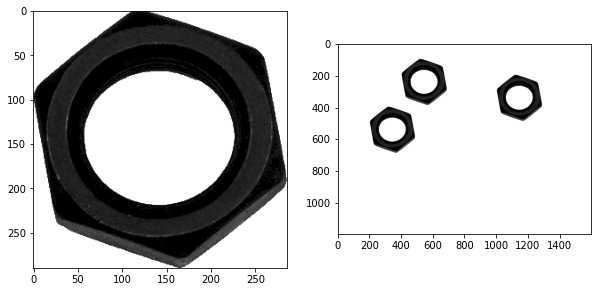
\includegraphics[scale=0.5]{figures/output_3_0.png}
    \end{figure}
  


\section{Part - I}

\hypertarget{otsus-thresholding}{%
\subsection{Otsu's thresholding}\label{otsus-thresholding}}

 Otsu's method avoids having to choose a value and determines an
  optimal global threshold value from the image histogram automatically.
  It is returned as the first output.


    \begin{tcolorbox}[breakable, size=fbox, boxrule=1pt, pad at break*=1mm,colback=cellbackground, colframe=cellborder]
\prompt{In}{incolor}{3}{\boxspacing}
\begin{Verbatim}[commandchars=\\\{\}]
\PY{n}{th\PYZus{}t}\PY{p}{,} \PY{n}{img\PYZus{}t} \PY{o}{=} \PY{n}{cv}\PY{o}{.}\PY{n}{threshold}\PY{p}{(}\PY{n}{template\PYZus{}im}\PY{p}{,}\PY{l+m+mi}{0}\PY{p}{,}\PY{l+m+mi}{255}\PY{p}{,}\PY{n}{cv}\PY{o}{.}\PY{n}{THRESH\PYZus{}BINARY\PYZus{}INV}\PY{o}{+}\PY{n}{cv}\PY{o}{.}\PY{n}{THRESH\PYZus{}OTSU}\PY{p}{)}
\PY{n}{th\PYZus{}b}\PY{p}{,} \PY{n}{img\PYZus{}b} \PY{o}{=} \PY{n}{cv}\PY{o}{.}\PY{n}{threshold}\PY{p}{(}\PY{n}{belt\PYZus{}im}\PY{p}{,}\PY{l+m+mi}{0}\PY{p}{,}\PY{l+m+mi}{255}\PY{p}{,}\PY{n}{cv}\PY{o}{.}\PY{n}{THRESH\PYZus{}BINARY\PYZus{}INV}\PY{o}{+}\PY{n}{cv}\PY{o}{.}\PY{n}{THRESH\PYZus{}OTSU}\PY{p}{)}
\end{Verbatim}
\end{tcolorbox}

    \hypertarget{morphological-closing}{%
\subsection{Morphological closing}\label{morphological-closing}}

Carrying out morphological closing to remove small holes inside the
foreground. Use a $3 \times 3$ kernel. Morphological closing is just dilation followed by erosion.

\begin{enumerate}
\def\labelenumi{\arabic{enumi}.}
\tightlist

\item
\textbf{Dilation}: a pixel element is `1' if atleast one pixel under the kernel
is `1'. So it increases the white region
\item
  \textbf{Erosion}: a pixel element is `1' if all the pixel under the kernel is
  `1'. So it decreases the white region

\end{enumerate}

    \begin{tcolorbox}[breakable, size=fbox, boxrule=1pt, pad at break*=1mm,colback=cellbackground, colframe=cellborder]
\prompt{In}{incolor}{4}{\boxspacing}
\begin{Verbatim}[commandchars=\\\{\}]
\PY{c+c1}{\PYZsh{} 3x3 matrix with all ones, with uint8 dtype}
\PY{n}{kernel} \PY{o}{=} \PY{n}{cv}\PY{o}{.}\PY{n}{getStructuringElement}\PY{p}{(}\PY{n}{cv}\PY{o}{.}\PY{n}{MORPH\PYZus{}RECT}\PY{p}{,} \PY{p}{(}\PY{l+m+mi}{3}\PY{p}{,}\PY{l+m+mi}{3}\PY{p}{)}\PY{p}{)}
\PY{n}{closing\PYZus{}t} \PY{o}{=} \PY{n}{cv}\PY{o}{.}\PY{n}{morphologyEx}\PY{p}{(}\PY{n}{img\PYZus{}t}\PY{p}{,} \PY{n}{cv}\PY{o}{.}\PY{n}{MORPH\PYZus{}CLOSE}\PY{p}{,} \PY{n}{kernel}\PY{p}{)} \PY{c+c1}{\PYZsh{} Dilation followed by Erosion}
\PY{n}{closing\PYZus{}b} \PY{o}{=} \PY{n}{cv}\PY{o}{.}\PY{n}{morphologyEx}\PY{p}{(}\PY{n}{img\PYZus{}b}\PY{p}{,} \PY{n}{cv}\PY{o}{.}\PY{n}{MORPH\PYZus{}CLOSE}\PY{p}{,} \PY{n}{kernel}\PY{p}{)} \PY{c+c1}{\PYZsh{} Dilation followed by Erosion}
\end{Verbatim}
\end{tcolorbox}

    \hypertarget{connected-component-analysis}{%
\subsection{Connected component
analysis}\label{connected-component-analysis}}

Apply the \texttt{cv.connectedComponentsWithStats} function

    \begin{tcolorbox}[breakable, size=fbox, boxrule=1pt, pad at break*=1mm,colback=cellbackground, colframe=cellborder]
\prompt{In}{incolor}{5}{\boxspacing}
\begin{Verbatim}[commandchars=\\\{\}]
\PY{n}{retval\PYZus{}t}\PY{p}{,} \PY{n}{labels\PYZus{}t}\PY{p}{,} \PY{n}{stats\PYZus{}t}\PY{p}{,} \PY{n}{centroids\PYZus{}t} \PY{o}{=} \PY{n}{cv}\PY{o}{.}\PY{n}{connectedComponentsWithStats}\PY{p}{(}\PY{n}{closing\PYZus{}t}\PY{p}{)}
\PY{n}{retval\PYZus{}b}\PY{p}{,} \PY{n}{labels\PYZus{}b}\PY{p}{,} \PY{n}{stats\PYZus{}b}\PY{p}{,} \PY{n}{centroids\PYZus{}b} \PY{o}{=} \PY{n}{cv}\PY{o}{.}\PY{n}{connectedComponentsWithStats}\PY{p}{(}\PY{n}{closing\PYZus{}b}\PY{p}{)}

\PY{k}{def} \PY{n+nf}{cca\PYZus{}stats}\PY{p}{(}\PY{n}{img\PYZus{}name}\PY{p}{,} \PY{n}{retval}\PY{p}{,} \PY{n}{labels}\PY{p}{,} \PY{n}{stats}\PY{p}{,} \PY{n}{centroids}\PY{p}{)}\PY{p}{:}
    \PY{n+nb}{print}\PY{p}{(}\PY{n}{img\PYZus{}name}\PY{o}{.}\PY{n}{center}\PY{p}{(}\PY{l+m+mi}{50}\PY{p}{,}\PY{l+s+s2}{\PYZdq{}}\PY{l+s+s2}{=}\PY{l+s+s2}{\PYZdq{}}\PY{p}{)}\PY{p}{)}
    \PY{n+nb}{print}\PY{p}{(}\PY{l+s+s2}{\PYZdq{}}\PY{l+s+s2}{Number of labels: }\PY{l+s+s2}{\PYZdq{}}\PY{p}{,} \PY{n}{retval}\PY{p}{)}
    \PY{n}{plt}\PY{o}{.}\PY{n}{imshow}\PY{p}{(}\PY{n}{labels}\PY{o}{.}\PY{n}{astype}\PY{p}{(}\PY{l+s+s1}{\PYZsq{}}\PY{l+s+s1}{uint8}\PY{l+s+s1}{\PYZsq{}}\PY{p}{)}\PY{p}{,} \PY{n}{cmap} \PY{o}{=}\PY{l+s+s1}{\PYZsq{}}\PY{l+s+s1}{gray}\PY{l+s+s1}{\PYZsq{}}\PY{p}{)}\PY{p}{;} \PY{n}{plt}\PY{o}{.}\PY{n}{show}\PY{p}{(}\PY{p}{)}
    \PY{n+nb}{print}\PY{p}{(}\PY{l+s+s2}{\PYZdq{}}\PY{l+s+s2}{Stats: }\PY{l+s+se}{\PYZbs{}n}\PY{l+s+s2}{\PYZdq{}}\PY{p}{,} \PY{n}{stats}\PY{p}{,}\PY{l+s+s1}{\PYZsq{}}\PY{l+s+se}{\PYZbs{}n}\PY{l+s+s1}{\PYZsq{}}\PY{p}{)} \PY{c+c1}{\PYZsh{} stats[label,cv.CC\PYZus{}STAT\PYZus{}quantity])}
    \PY{n+nb}{print}\PY{p}{(}\PY{l+s+s2}{\PYZdq{}}\PY{l+s+s2}{Centroids: }\PY{l+s+se}{\PYZbs{}n}\PY{l+s+s2}{\PYZdq{}}\PY{p}{,} \PY{n}{centroids}\PY{p}{,}\PY{l+s+s1}{\PYZsq{}}\PY{l+s+se}{\PYZbs{}n}\PY{l+s+s1}{\PYZsq{}}\PY{p}{)}

\PY{n}{cca\PYZus{}stats}\PY{p}{(}\PY{l+s+s2}{\PYZdq{}}\PY{l+s+s2}{Template Image}\PY{l+s+s2}{\PYZdq{}}\PY{p}{,} \PY{n}{retval\PYZus{}t}\PY{p}{,} \PY{n}{labels\PYZus{}t}\PY{p}{,} \PY{n}{stats\PYZus{}t}\PY{p}{,} \PY{n}{centroids\PYZus{}t}\PY{p}{)}
\PY{n}{cca\PYZus{}stats}\PY{p}{(}\PY{l+s+s2}{\PYZdq{}}\PY{l+s+s2}{Belt Image}\PY{l+s+s2}{\PYZdq{}}\PY{p}{,} \PY{n}{retval\PYZus{}b}\PY{p}{,} \PY{n}{labels\PYZus{}b}\PY{p}{,} \PY{n}{stats\PYZus{}b}\PY{p}{,} \PY{n}{centroids\PYZus{}b}\PY{p}{)}
\end{Verbatim}
\end{tcolorbox}

\begin{figure}[!h]
	\centering
	\subfigure[Template Image]
	{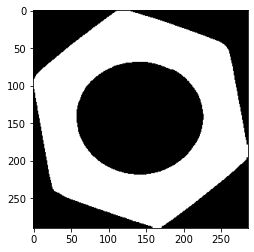
\includegraphics[scale=0.5]{figures/output_9_1.png}
	}
	\subfigure[Belt Image]
	{ 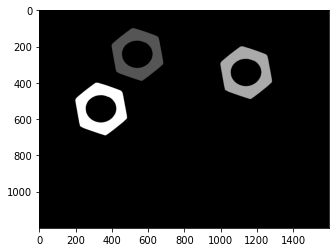
\includegraphics[scale=0.5]{figures/output_9_3.png}
	}
\end{figure}


    \begin{Verbatim}[commandchars=\\\{\}]
==================Template Image==================
Number of labels:  2
    \end{Verbatim}


    \begin{Verbatim}[commandchars=\\\{\}]
Stats:
 [[    0     0   286   290 42290]
 [    0     0   286   290 40650]]

Centroids:
 [[142.18770395 145.19172381]
 [142.82489545 143.780369  ]]

====================Belt Image====================
Number of labels:  4
    \end{Verbatim}


    \begin{Verbatim}[commandchars=\\\{\}]
Stats:
 [[      0       0    1600    1200 1798161]
 [    400     100     286     290   40613]
 [   1000     200     286     290   40613]
 [    200     400     286     290   40613]]

Centroids:
 [[ 807.85728475  614.56805258]
 [ 542.82567158  243.78479797]
 [1142.82567158  343.78479797]
 [ 342.82567158  543.78479797]]

    \end{Verbatim}

    \begin{enumerate}
\item
  How many connected components are detected in each image?\\
  \textbf{Template Image} = 2 (\emph{including background})\\ \textbf{Belt
  Image} = 4 (\emph{including background})
\item
  What are the statistics? Interpret these statistics. \\ Statistics are
  properties related to each connected component. Statistics object is a
  2D array where each column represent a different quantity related to a
  given connected component as described below.
  	\begin{itemize}
  		\item \textbf{Column 1:} \emph{cv.CC\_STAT\_LEFT}: the leftmost (x) coordinate
  		which is the inclusive start of the bounding box in the horizontal
  		direction.
  		\item \textbf{Column 2:} \emph{cv.CC\_STAT\_TOP}: the topmost (y)
  		coordinate which is the inclusive start of the bounding box in the
  		vertical direction.
  		\item \textbf{Column 3:} \emph{cv.CC\_STAT\_WIDTH}: the
  		horizontal size of the bounding box.
  		\item \textbf{Column 4:}
  		\emph{cv.CC\_STAT\_HEIGHT}: the vertical size of the bounding box.
  		\item \textbf{Column 5:} \emph{cv.CC\_STAT\_AREA}: the total area (in pixels)
  		of the connected component.
  	\end{itemize}

  \item
  What are the centroids?\\ Each row of the 2D \texttt{Cenroids} obejct
  represents the (x,y) coordinates of centroid of the corresponding
  connected component.
\end{enumerate}





    \hypertarget{contour-analysis}{%
\subsection{Contour analysis}\label{contour-analysis}}

Use \texttt{cv.findContours} function to retrieve the \emph{extreme outer}
contours.\\

The functions output contours is a Python list of all the contours in the image. Each
individual contour is a Numpy array of (x,y) coordinates of boundary
points of the object. Display these countours.

    \begin{tcolorbox}[breakable, size=fbox, boxrule=1pt, pad at break*=1mm,colback=cellbackground, colframe=cellborder]
\prompt{In}{incolor}{6}{\boxspacing}
\begin{Verbatim}[commandchars=\\\{\}]
\PY{c+c1}{\PYZsh{} cv.RETR\PYZus{}EXTERNAL retrieve only the extreme outer contours}
\PY{n}{contours\PYZus{}t}\PY{p}{,}\PY{n}{\PYZus{}} \PY{o}{=} \PY{n}{cv}\PY{o}{.}\PY{n}{findContours}\PY{p}{(}\PY{n}{closing\PYZus{}t}\PY{p}{,} \PY{n}{cv}\PY{o}{.}\PY{n}{RETR\PYZus{}EXTERNAL}\PY{p}{,} \PY{n}{cv}\PY{o}{.}\PY{n}{CHAIN\PYZus{}APPROX\PYZus{}SIMPLE}\PY{p}{)}
\PY{n}{contours\PYZus{}b}\PY{p}{,}\PY{n}{\PYZus{}} \PY{o}{=} \PY{n}{cv}\PY{o}{.}\PY{n}{findContours}\PY{p}{(}\PY{n}{closing\PYZus{}b}\PY{p}{,} \PY{n}{cv}\PY{o}{.}\PY{n}{RETR\PYZus{}EXTERNAL}\PY{p}{,} \PY{n}{cv}\PY{o}{.}\PY{n}{CHAIN\PYZus{}APPROX\PYZus{}SIMPLE}\PY{p}{)}

\PY{c+c1}{\PYZsh{} Visualizing contours (\PYZhy{}1 argument to plot all the contours)}
\PY{n}{im\PYZus{}contours\PYZus{}belt} \PY{o}{=} \PY{n}{np}\PY{o}{.}\PY{n}{zeros}\PY{p}{(}\PY{p}{(}\PY{n}{belt\PYZus{}im}\PY{o}{.}\PY{n}{shape}\PY{p}{[}\PY{l+m+mi}{0}\PY{p}{]}\PY{p}{,}\PY{n}{belt\PYZus{}im}\PY{o}{.}\PY{n}{shape}\PY{p}{[}\PY{l+m+mi}{1}\PY{p}{]}\PY{p}{,}\PY{l+m+mi}{3}\PY{p}{)}\PY{p}{,} \PY{n}{np}\PY{o}{.}\PY{n}{uint8}\PY{p}{)}
\PY{n}{conts} \PY{o}{=} \PY{n}{cv}\PY{o}{.}\PY{n}{drawContours}\PY{p}{(}\PY{n}{im\PYZus{}contours\PYZus{}belt}\PY{p}{,} \PY{n}{contours\PYZus{}b}\PY{p}{,} \PY{o}{\PYZhy{}}\PY{l+m+mi}{1}\PY{p}{,} \PY{p}{(}\PY{l+m+mi}{0}\PY{p}{,}\PY{l+m+mi}{255}\PY{p}{,}\PY{l+m+mi}{0}\PY{p}{)}\PY{p}{,} \PY{l+m+mi}{3}\PY{p}{)}\PY{o}{.}\PY{n}{astype}\PY{p}{(}\PY{l+s+s1}{\PYZsq{}}\PY{l+s+s1}{uint8}\PY{l+s+s1}{\PYZsq{}}\PY{p}{)}
\PY{n}{plt}\PY{o}{.}\PY{n}{imshow}\PY{p}{(}\PY{n}{conts}\PY{p}{)}\PY{p}{,} \PY{n}{plt}\PY{o}{.}\PY{n}{show}\PY{p}{(}\PY{p}{)}
\end{Verbatim}
\end{tcolorbox}

    \begin{figure}[!h]
		\centering
    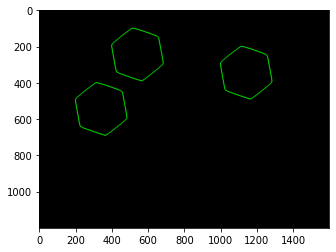
\includegraphics[scale=0.7]{figures/output_12_0.png}
    \end{figure}
    { \hspace*{\fill} \\}



    \hypertarget{count-the-number-of-matching-hexagonal-nuts-in-belt.png.}{%
\subsection{\texorpdfstring{Count the number of matching hexagonal
nuts in
\texttt{belt.png}.}{Count the number of matching hexagonal nuts in belt.png.}}\label{count-the-number-of-matching-hexagonal-nuts-in-belt.png.}}

\texttt{cv.matchShapes} function enables us to compare two shapes, or
two contours and returns a metric showing the similarity. The lower the
result, the better match it is.
\texttt{retval=cv.matchShapes(contour1,\ contour2,\ method,\ parameter)}

    \begin{tcolorbox}[breakable, size=fbox, boxrule=1pt, pad at break*=1mm,colback=cellbackground, colframe=cellborder]
\prompt{In}{incolor}{7}{\boxspacing}
\begin{Verbatim}[commandchars=\\\{\}]
\PY{n}{label} \PY{o}{=} \PY{l+m+mi}{1} \PY{c+c1}{\PYZsh{} remember that the label of the background is 0}
\PY{n}{belt} \PY{o}{=} \PY{p}{(}\PY{p}{(}\PY{n}{labels\PYZus{}b} \PY{o}{\PYZgt{}}\PY{o}{=} \PY{n}{label}\PY{p}{)}\PY{o}{*}\PY{l+m+mi}{255}\PY{p}{)}\PY{o}{.}\PY{n}{astype}\PY{p}{(}\PY{l+s+s1}{\PYZsq{}}\PY{l+s+s1}{uint8}\PY{l+s+s1}{\PYZsq{}}\PY{p}{)}
\PY{n}{plt}\PY{o}{.}\PY{n}{imshow}\PY{p}{(}\PY{n}{belt}\PY{p}{,} \PY{n}{cmap} \PY{o}{=}\PY{l+s+s1}{\PYZsq{}}\PY{l+s+s1}{gray}\PY{l+s+s1}{\PYZsq{}}\PY{p}{)}\PY{p}{,}\PY{n}{plt}\PY{o}{.}\PY{n}{show}\PY{p}{(}\PY{p}{)}
\PY{n}{belt\PYZus{}cont}\PY{p}{,}\PY{n}{\PYZus{}} \PY{o}{=} \PY{n}{cv}\PY{o}{.}\PY{n}{findContours}\PY{p}{(}\PY{n}{belt}\PY{p}{,} \PY{n}{cv}\PY{o}{.}\PY{n}{RETR\PYZus{}EXTERNAL}\PY{p}{,} \PY{n}{cv}\PY{o}{.}\PY{n}{CHAIN\PYZus{}APPROX\PYZus{}SIMPLE}\PY{p}{)}
\PY{k}{for} \PY{n}{j}\PY{p}{,}\PY{n}{c} \PY{o+ow}{in} \PY{n+nb}{enumerate}\PY{p}{(}\PY{n}{belt\PYZus{}cont}\PY{p}{)}\PY{p}{:}
        \PY{n+nb}{print}\PY{p}{(}\PY{l+s+s2}{\PYZdq{}}\PY{l+s+s2}{Contour }\PY{l+s+s2}{\PYZdq{}}\PY{p}{,} \PY{n}{j} \PY{o}{+}\PY{l+m+mi}{1}\PY{p}{,}\PY{l+s+s2}{\PYZdq{}}\PY{l+s+s2}{\PYZhy{}\PYZhy{}\PYZgt{}}\PY{l+s+s2}{\PYZdq{}}\PY{p}{,} \PY{n}{cv}\PY{o}{.}\PY{n}{matchShapes}\PY{p}{(}\PY{n}{contours\PYZus{}t}\PY{p}{[}\PY{l+m+mi}{0}\PY{p}{]}\PY{p}{,} \PY{n}{c}\PY{p}{,} \PY{n}{cv}\PY{o}{.}\PY{n}{CONTOURS\PYZus{}MATCH\PYZus{}I1}\PY{p}{,} \PY{l+m+mf}{0.0}\PY{p}{)}\PY{p}{)}
\end{Verbatim}
\end{tcolorbox}

    \begin{figure}[!h]
		\centering
    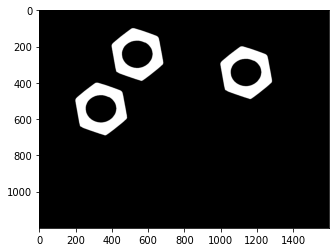
\includegraphics[scale=0.7]{figures/output_14_0.png}
    \end{figure}
    { \hspace*{\fill} \\}

    \begin{Verbatim}[commandchars=\\\{\}]
Contour  1 --> 0.00010071698397173812
Contour  2 --> 0.00010071698397950968
Contour  3 --> 0.00010071698397506879
    \end{Verbatim}

    \hypertarget{part---ii}{%
\section{Part - II}\label{part---ii}}

\hypertarget{frame-tracking-through-image-moments.}{%
\subsection{Frame tracking through image
moments.}\label{frame-tracking-through-image-moments.}}

Use the \texttt{cv.contourArea()} to calculate the the area of the \texttt{contours\_b{[}1{]}}

    \begin{tcolorbox}[breakable, size=fbox, boxrule=1pt, pad at break*=1mm,colback=cellbackground, colframe=cellborder]
\prompt{In}{incolor}{8}{\boxspacing}
\begin{Verbatim}[commandchars=\\\{\}]
\PY{n}{ca} \PY{o}{=} \PY{n}{cv}\PY{o}{.}\PY{n}{contourArea}\PY{p}{(}\PY{n}{contours\PYZus{}b}\PY{p}{[}\PY{l+m+mi}{1}\PY{p}{]}\PY{p}{)}
\PY{n+nb}{print}\PY{p}{(}\PY{n}{ca}\PY{p}{)}
\end{Verbatim}
\end{tcolorbox}

    \begin{Verbatim}[commandchars=\\\{\}]
60059.5
    \end{Verbatim}

    Use the \texttt{cv.moments} to extract the x and y coordinates of the
centroid of \texttt{contours\_b{[}1{]}}.

    \begin{tcolorbox}[breakable, size=fbox, boxrule=1pt, pad at break*=1mm,colback=cellbackground, colframe=cellborder]
\prompt{In}{incolor}{9}{\boxspacing}
\begin{Verbatim}[commandchars=\\\{\}]
\PY{n}{M} \PY{o}{=} \PY{n}{cv}\PY{o}{.}\PY{n}{moments}\PY{p}{(}\PY{n}{contours\PYZus{}b}\PY{p}{[}\PY{l+m+mi}{1}\PY{p}{]}\PY{p}{)}
\PY{n+nb}{print}\PY{p}{(}\PY{l+s+s2}{\PYZdq{}}\PY{l+s+s2}{Area = }\PY{l+s+s2}{\PYZdq{}}\PY{p}{,} \PY{n}{M}\PY{p}{[}\PY{l+s+s1}{\PYZsq{}}\PY{l+s+s1}{m00}\PY{l+s+s1}{\PYZsq{}}\PY{p}{]}\PY{p}{)}

\PY{n}{cx}\PY{p}{,} \PY{n}{cy} \PY{o}{=} \PY{n+nb}{int}\PY{p}{(}\PY{n}{M}\PY{p}{[}\PY{l+s+s1}{\PYZsq{}}\PY{l+s+s1}{m10}\PY{l+s+s1}{\PYZsq{}}\PY{p}{]}\PY{o}{/}\PY{n}{M}\PY{p}{[}\PY{l+s+s1}{\PYZsq{}}\PY{l+s+s1}{m00}\PY{l+s+s1}{\PYZsq{}}\PY{p}{]}\PY{p}{)}\PY{p}{,} \PY{n+nb}{int}\PY{p}{(}\PY{n}{M}\PY{p}{[}\PY{l+s+s1}{\PYZsq{}}\PY{l+s+s1}{m01}\PY{l+s+s1}{\PYZsq{}}\PY{p}{]}\PY{o}{/}\PY{n}{M}\PY{p}{[}\PY{l+s+s1}{\PYZsq{}}\PY{l+s+s1}{m00}\PY{l+s+s1}{\PYZsq{}}\PY{p}{]}\PY{p}{)}
\PY{n+nb}{print}\PY{p}{(}\PY{l+s+s2}{\PYZdq{}}\PY{l+s+s2}{Centroid = (}\PY{l+s+si}{\PYZob{}\PYZcb{}}\PY{l+s+s2}{, }\PY{l+s+si}{\PYZob{}\PYZcb{}}\PY{l+s+s2}{)}\PY{l+s+s2}{\PYZdq{}}\PY{o}{.}\PY{n}{format}\PY{p}{(}\PY{n}{cx}\PY{p}{,}\PY{n}{cy}\PY{p}{)}\PY{p}{)}
\end{Verbatim}
\end{tcolorbox}

    \begin{Verbatim}[commandchars=\\\{\}]
Area =  60059.5
Centroid = (1142, 343)
    \end{Verbatim}

    Make a variable called \texttt{count} to represent the number of
contours and set it to the value 1. Make an np array {[}cx, cy, ca,
count{]} and name this as \texttt{object\_prev\_frame}.

    \begin{tcolorbox}[breakable, size=fbox, boxrule=1pt, pad at break*=1mm,colback=cellbackground, colframe=cellborder]
\prompt{In}{incolor}{10}{\boxspacing}
\begin{Verbatim}[commandchars=\\\{\}]
\PY{n}{count} \PY{o}{=} \PY{l+m+mi}{1}
\PY{n}{object\PYZus{}prev\PYZus{}frame} \PY{o}{=} \PY{n}{np}\PY{o}{.}\PY{n}{array}\PY{p}{(}\PY{p}{[}\PY{n}{cx}\PY{p}{,} \PY{n}{cy}\PY{p}{,} \PY{n}{ca}\PY{p}{,} \PY{n}{count}\PY{p}{]}\PY{p}{)}
\end{Verbatim}
\end{tcolorbox}

    Similarly, you can create the \texttt{object\_curr\_frame}(to describe
the current values) and define the threshold \texttt{delta\_x} to check
whether the corresponding element of both the
\texttt{object\_curr\_frame} and \texttt{object\_prev\_frame} are less
than the \texttt{delta\_x}. You can set \texttt{delta\_x} as 15 or so.
(Here the \texttt{delta\_x} can be thought of as the movement of the cx
from frame to frame)

    \begin{tcolorbox}[breakable, size=fbox, boxrule=1pt, pad at break*=1mm,colback=cellbackground, colframe=cellborder]
\prompt{In}{incolor}{11}{\boxspacing}
\begin{Verbatim}[commandchars=\\\{\}]
\PY{n}{delta\PYZus{}x} \PY{o}{=} \PY{l+m+mi}{15}
\end{Verbatim}
\end{tcolorbox}

    \hypertarget{part---iii}{%
\section{Part - III}\label{part---iii}}

\hypertarget{implement-the-function-get_indexed_image-which-takes-an-image-as-the-input-performs-thresholding-closing-and-connected-component-analysis-and-return-retval-labels-stats-centroids.-grading}{%
\subsection{\texorpdfstring{1. Implement the function
\texttt{get\_indexed\_image}, which takes an image as the input,
performs thresholding, closing, and connected component analysis and
return retval, labels, stats, centroids.
(Grading)}{1. Implement the function get\_indexed\_image, which takes an image as the input, performs thresholding, closing, and connected component analysis and return retval, labels, stats, centroids. (Grading)}}\label{implement-the-function-get_indexed_image-which-takes-an-image-as-the-input-performs-thresholding-closing-and-connected-component-analysis-and-return-retval-labels-stats-centroids.-grading}}

    \begin{tcolorbox}[breakable, size=fbox, boxrule=1pt, pad at break*=1mm,colback=cellbackground, colframe=cellborder]
\prompt{In}{incolor}{12}{\boxspacing}
\begin{Verbatim}[commandchars=\\\{\}]
\PY{k}{def} \PY{n+nf}{get\PYZus{}indexed\PYZus{}image}\PY{p}{(}\PY{n}{im}\PY{p}{)}\PY{p}{:}
    \PY{l+s+sd}{\PYZdq{}\PYZdq{}\PYZdq{} Thresholding, closing, and connected component analysis lumped}
\PY{l+s+sd}{    \PYZdq{}\PYZdq{}\PYZdq{}}

    \PY{n}{\PYZus{}}\PY{p}{,} \PY{n}{img} \PY{o}{=} \PY{n}{cv}\PY{o}{.}\PY{n}{threshold}\PY{p}{(}\PY{n}{im}\PY{p}{,}\PY{l+m+mi}{0}\PY{p}{,}\PY{l+m+mi}{255}\PY{p}{,}\PY{n}{cv}\PY{o}{.}\PY{n}{THRESH\PYZus{}BINARY\PYZus{}INV}\PY{o}{+}\PY{n}{cv}\PY{o}{.}\PY{n}{THRESH\PYZus{}OTSU}\PY{p}{)}
    \PY{n}{kernel} \PY{o}{=} \PY{n}{cv}\PY{o}{.}\PY{n}{getStructuringElement}\PY{p}{(}\PY{n}{cv}\PY{o}{.}\PY{n}{MORPH\PYZus{}RECT}\PY{p}{,} \PY{p}{(}\PY{l+m+mi}{3}\PY{p}{,}\PY{l+m+mi}{3}\PY{p}{)}\PY{p}{)}
    \PY{n}{closing} \PY{o}{=} \PY{n}{cv}\PY{o}{.}\PY{n}{morphologyEx}\PY{p}{(}\PY{n}{img}\PY{p}{,} \PY{n}{cv}\PY{o}{.}\PY{n}{MORPH\PYZus{}CLOSE}\PY{p}{,} \PY{n}{kernel}\PY{p}{)} \PY{c+c1}{\PYZsh{} Dilation followed by Erosion}
    \PY{n}{retval}\PY{p}{,} \PY{n}{labels}\PY{p}{,} \PY{n}{stats}\PY{p}{,} \PY{n}{centroids} \PY{o}{=} \PY{n}{cv}\PY{o}{.}\PY{n}{connectedComponentsWithStats}\PY{p}{(}\PY{n}{closing}\PY{p}{)}

    \PY{k}{return} \PY{n}{retval}\PY{p}{,} \PY{n}{labels}\PY{p}{,} \PY{n}{stats}\PY{p}{,} \PY{n}{centroids}
\end{Verbatim}
\end{tcolorbox}

    \hypertarget{implement-the-function-is_new-which-checks-the-dissimilarity-between-2-vectors.-grading}{%
\subsection{\texorpdfstring{2. Implement the function
\texttt{is\_new}, which checks the dissimilarity between 2 vectors.
(Grading)}{2. Implement the function is\_new, which checks the dissimilarity between 2 vectors. (Grading)}}\label{implement-the-function-is_new-which-checks-the-dissimilarity-between-2-vectors.-grading}}

    \begin{tcolorbox}[breakable, size=fbox, boxrule=1pt, pad at break*=1mm,colback=cellbackground, colframe=cellborder]
\prompt{In}{incolor}{13}{\boxspacing}
\begin{Verbatim}[commandchars=\\\{\}]
\PY{k}{def} \PY{n+nf}{is\PYZus{}new}\PY{p}{(}\PY{n}{a}\PY{p}{,} \PY{n}{b}\PY{p}{,} \PY{n}{delta}\PY{p}{,} \PY{n}{i}\PY{p}{)}\PY{p}{:}
    \PY{l+s+sd}{\PYZdq{}\PYZdq{}\PYZdq{} Vector Dissimilarity with an Array of Vectors}
\PY{l+s+sd}{    Checks if vector b is similar to a one or more vectors in a outside the tolerances specified in delta. }
\PY{l+s+sd}{    vector i specifies which elements in b to compare with those in a. }
\PY{l+s+sd}{    \PYZdq{}\PYZdq{}\PYZdq{}}

    \PY{n}{absolute\PYZus{}different} \PY{o}{=} \PY{n}{np}\PY{o}{.}\PY{n}{abs}\PY{p}{(}\PY{n}{a} \PY{o}{\PYZhy{}} \PY{n}{b}\PY{p}{)} \PY{c+c1}{\PYZsh{} getting the absolute differences}
    \PY{n}{states} \PY{o}{=} \PY{p}{[}\PY{p}{]} \PY{c+c1}{\PYZsh{} arry to store result of each column}
    \PY{k}{for} \PY{n}{element} \PY{o+ow}{in} \PY{n}{i}\PY{p}{:}
        \PY{c+c1}{\PYZsh{} compare each value in ith column with the specified delta}
        \PY{n}{absolute\PYZus{}different}\PY{p}{[}\PY{p}{:}\PY{p}{,}\PY{n}{element}\PY{p}{]} \PY{o}{=} \PY{p}{(}\PY{n}{absolute\PYZus{}different}\PY{p}{[}\PY{p}{:}\PY{p}{,}\PY{n}{element}\PY{p}{]} \PY{o}{\PYZgt{}} \PY{n}{delta}\PY{p}{[}\PY{n}{element}\PY{p}{]}\PY{p}{)}
        \PY{c+c1}{\PYZsh{} check whether the condition is true for all the values in that column}
        \PY{n}{states}\PY{o}{.}\PY{n}{append}\PY{p}{(}\PY{n}{absolute\PYZus{}different}\PY{p}{[}\PY{p}{:}\PY{p}{,}\PY{n}{element}\PY{p}{]}\PY{o}{.}\PY{n}{all}\PY{p}{(}\PY{p}{)}\PY{p}{)}

    \PY{l+s+s1}{\PYZsq{}}\PY{l+s+s1}{Check whether the absolute different between all the elements of ith column of each array is greater than the ith delta value (See thee example in the next cell)}\PY{l+s+s1}{\PYZsq{}}
    \PY{c+c1}{\PYZsh{} summarize the results of each column to get the final result.}
    \PY{n}{state} \PY{o}{=} \PY{n}{np}\PY{o}{.}\PY{n}{array}\PY{p}{(}\PY{n}{states}\PY{p}{)}\PY{o}{.}\PY{n}{all}\PY{p}{(}\PY{p}{)}

    \PY{k}{return} \PY{n}{state}
\end{Verbatim}
\end{tcolorbox}
\pagebreak
    \begin{tcolorbox}[breakable, size=fbox, boxrule=1pt, pad at break*=1mm,colback=cellbackground, colframe=cellborder]
\prompt{In}{incolor}{14}{\boxspacing}
\begin{Verbatim}[commandchars=\\\{\}]
\PY{c+c1}{\PYZsh{} check is\PYZus{}new  expected answer False}
\PY{n}{a} \PY{o}{=} \PY{n}{np}\PY{o}{.}\PY{n}{array}\PY{p}{(}\PY{p}{[}\PY{p}{[}\PY{l+m+mf}{1.36100e+03}\PY{p}{,} \PY{l+m+mf}{5.53000e+02}\PY{p}{,} \PY{l+m+mf}{5.99245e+04}\PY{p}{,} \PY{l+m+mf}{2.00000e+00}\PY{p}{]}\PY{p}{,}
              \PY{p}{[}\PY{l+m+mf}{7.61000e+02}\PY{p}{,} \PY{l+m+mf}{4.53000e+02}\PY{p}{,} \PY{l+m+mf}{5.99385e+04}\PY{p}{,} \PY{l+m+mf}{1.00000e+00}\PY{p}{]}\PY{p}{,}
              \PY{p}{[}\PY{l+m+mf}{1.55200e+03}\PY{p}{,} \PY{l+m+mf}{2.43000e+02}\PY{p}{,} \PY{l+m+mf}{6.00585e+04}\PY{p}{,} \PY{l+m+mf}{3.00000e+00}\PY{p}{]}\PY{p}{]}\PY{p}{)}

\PY{n}{b} \PY{o}{=} \PY{n}{np}\PY{o}{.}\PY{n}{array}\PY{p}{(} \PY{p}{[}\PY{l+m+mf}{7.51000e+02}\PY{p}{,} \PY{l+m+mf}{4.53000e+02}\PY{p}{,} \PY{l+m+mf}{5.99385e+04}\PY{p}{,} \PY{l+m+mf}{3.00000e+00}\PY{p}{]}\PY{p}{)}
\PY{n}{delta} \PY{o}{=} \PY{n}{np}\PY{o}{.}\PY{n}{array}\PY{p}{(}\PY{p}{[}\PY{n}{delta\PYZus{}x}\PY{p}{]}\PY{p}{)}
\PY{n}{i} \PY{o}{=} \PY{n}{np}\PY{o}{.}\PY{n}{array}\PY{p}{(}\PY{p}{[}\PY{l+m+mi}{0}\PY{p}{]}\PY{p}{)}

\PY{k}{assert} \PY{n}{is\PYZus{}new}\PY{p}{(}\PY{n}{a}\PY{p}{,} \PY{n}{b}\PY{p}{,} \PY{n}{delta}\PY{p}{,} \PY{n}{i}\PY{p}{)} \PY{o}{==} \PY{k+kc}{False}\PY{p}{,} \PY{l+s+s2}{\PYZdq{}}\PY{l+s+s2}{ Check the function }\PY{l+s+s2}{\PYZdq{}}
\end{Verbatim}
\end{tcolorbox}

    \hypertarget{if-the-array-a-is-in-the-shape-of-number-of-nuts-lenobject_prev_frame-i.e.-array-a-is-made-by-stacking-all-the-object_prev_frame-for-each-frame.-if-b-is-in-the-form-of-cx-cy-ca-count-write-the-function-prev_index-to-find-the-index-of-a-particular-nut-in-the-previous-frame.-grading}{%
\subsection{\texorpdfstring{3. If the array \texttt{a} is in the
shape of (number of nuts , len(object\_prev\_frame)) ( i.e.~array
\texttt{a} is made by stacking all the \texttt{object\_prev\_frame} for
each frame. If b is in the form of {[}cx, cy, ca, count{]}, write the
function \texttt{prev\_index} to find the index of a particular nut in
the previous frame.
(Grading)}{3. If the array a is in the shape of (number of nuts , len(object\_prev\_frame)) ( i.e.~array a is made by stacking all the object\_prev\_frame for each frame. If b is in the form of {[}cx, cy, ca, count{]}, write the function prev\_index to find the index of a particular nut in the previous frame. (Grading)}}\label{if-the-array-a-is-in-the-shape-of-number-of-nuts-lenobject_prev_frame-i.e.-array-a-is-made-by-stacking-all-the-object_prev_frame-for-each-frame.-if-b-is-in-the-form-of-cx-cy-ca-count-write-the-function-prev_index-to-find-the-index-of-a-particular-nut-in-the-previous-frame.-grading}}

    \begin{tcolorbox}[breakable, size=fbox, boxrule=1pt, pad at break*=1mm,colback=cellbackground, colframe=cellborder]
\prompt{In}{incolor}{15}{\boxspacing}
\begin{Verbatim}[commandchars=\\\{\}]
\PY{k}{def} \PY{n+nf}{prev\PYZus{}index}\PY{p}{(}\PY{n}{a}\PY{p}{,} \PY{n}{b}\PY{p}{,} \PY{n}{delta}\PY{p}{,} \PY{n}{i}\PY{p}{)}\PY{p}{:}
    \PY{l+s+sd}{\PYZdq{}\PYZdq{}\PYZdq{} Returns Previous Index}
\PY{l+s+sd}{    Returns the index of the apppearance of the object in the previous frame.}
\PY{l+s+sd}{    (See thee example in the next cell)}
\PY{l+s+sd}{    \PYZdq{}\PYZdq{}\PYZdq{}}
    \PY{n}{index} \PY{o}{=} \PY{o}{\PYZhy{}}\PY{l+m+mi}{1}
    \PY{n}{absolute\PYZus{}different} \PY{o}{=} \PY{n}{np}\PY{o}{.}\PY{n}{absolute}\PY{p}{(}\PY{n}{a} \PY{o}{\PYZhy{}} \PY{n}{b}\PY{p}{)}
    \PY{n}{matching\PYZus{}rows} \PY{o}{=} \PY{p}{[}\PY{p}{]}
    \PY{k}{for} \PY{n}{element} \PY{o+ow}{in} \PY{n}{i}\PY{p}{:}
        \PY{n}{absolute\PYZus{}different}\PY{p}{[}\PY{p}{:}\PY{p}{,}\PY{n}{element}\PY{p}{]} \PY{o}{=} \PY{p}{(}\PY{n}{absolute\PYZus{}different}\PY{p}{[}\PY{p}{:}\PY{p}{,}\PY{n}{element}\PY{p}{]} \PY{o}{\PYZlt{}}\PY{o}{=} \PY{n}{delta}\PY{p}{[}\PY{n}{element}\PY{p}{]}\PY{p}{)}
        \PY{c+c1}{\PYZsh{} find the row where the above condition is true.}
        \PY{n}{matching\PYZus{}row} \PY{o}{=} \PY{n}{np}\PY{o}{.}\PY{n}{where}\PY{p}{(}\PY{n}{absolute\PYZus{}different}\PY{p}{[}\PY{p}{:}\PY{p}{,}\PY{n}{element}\PY{p}{]}\PY{p}{)}\PY{p}{[}\PY{l+m+mi}{0}\PY{p}{]}
        \PY{n}{matching\PYZus{}rows}\PY{o}{.}\PY{n}{append}\PY{p}{(}\PY{n}{matching\PYZus{}row}\PY{p}{)}

    \PY{c+c1}{\PYZsh{} get the best match out of all the matches}
    \PY{n}{values}\PY{p}{,} \PY{n}{counts} \PY{o}{=} \PY{n}{np}\PY{o}{.}\PY{n}{unique}\PY{p}{(}\PY{n}{matching\PYZus{}rows}\PY{p}{,} \PY{n}{return\PYZus{}counts}\PY{o}{=}\PY{k+kc}{True}\PY{p}{)}
    \PY{n}{best\PYZus{}match} \PY{o}{=} \PY{n}{values}\PY{p}{[}\PY{n}{np}\PY{o}{.}\PY{n}{argmax}\PY{p}{(}\PY{n}{counts}\PY{p}{)}\PY{p}{]}

    \PY{n}{matching\PYZus{}nut} \PY{o}{=} \PY{n}{a}\PY{p}{[}\PY{n}{best\PYZus{}match}\PY{p}{]}
    \PY{n}{index} \PY{o}{=} \PY{n}{matching\PYZus{}nut}\PY{p}{[}\PY{o}{\PYZhy{}}\PY{l+m+mi}{1}\PY{p}{]} \PY{c+c1}{\PYZsh{} since count keeps the index of a nut.}

    \PY{k}{return} \PY{n}{index}
\end{Verbatim}
\end{tcolorbox}

    \begin{tcolorbox}[breakable, size=fbox, boxrule=1pt, pad at break*=1mm,colback=cellbackground, colframe=cellborder]
\prompt{In}{incolor}{16}{\boxspacing}
\begin{Verbatim}[commandchars=\\\{\}]
\PY{c+c1}{\PYZsh{} check prev\PYZus{}index  expected answer 1}
\PY{n}{a} \PY{o}{=} \PY{n}{np}\PY{o}{.}\PY{n}{array}\PY{p}{(}\PY{p}{[}\PY{p}{[}\PY{l+m+mf}{1.36100e+03}\PY{p}{,} \PY{l+m+mf}{5.53000e+02}\PY{p}{,} \PY{l+m+mf}{5.99245e+04}\PY{p}{,} \PY{l+m+mf}{2.00000e+00}\PY{p}{]}\PY{p}{,}
              \PY{p}{[}\PY{l+m+mf}{7.61000e+02}\PY{p}{,} \PY{l+m+mf}{4.53000e+02}\PY{p}{,} \PY{l+m+mf}{5.99385e+04}\PY{p}{,} \PY{l+m+mf}{1.00000e+00}\PY{p}{]}\PY{p}{,}
              \PY{p}{[}\PY{l+m+mf}{1.55200e+03}\PY{p}{,} \PY{l+m+mf}{2.43000e+02}\PY{p}{,} \PY{l+m+mf}{6.00585e+04}\PY{p}{,} \PY{l+m+mf}{3.00000e+00}\PY{p}{]}\PY{p}{]}\PY{p}{)}

\PY{n}{b} \PY{o}{=} \PY{n}{np}\PY{o}{.}\PY{n}{array}\PY{p}{(} \PY{p}{[}\PY{l+m+mf}{7.51000e+02}\PY{p}{,} \PY{l+m+mf}{4.53000e+02}\PY{p}{,} \PY{l+m+mf}{5.99385e+04}\PY{p}{,} \PY{l+m+mf}{3.00000e+00}\PY{p}{]}\PY{p}{)}
\PY{n}{delta} \PY{o}{=} \PY{n}{np}\PY{o}{.}\PY{n}{array}\PY{p}{(}\PY{p}{[}\PY{n}{delta\PYZus{}x}\PY{p}{]}\PY{p}{)}
\PY{n}{i} \PY{o}{=} \PY{n}{np}\PY{o}{.}\PY{n}{array}\PY{p}{(}\PY{p}{[}\PY{l+m+mi}{0}\PY{p}{]}\PY{p}{)}

\PY{k}{assert} \PY{n}{prev\PYZus{}index}\PY{p}{(}\PY{n}{a}\PY{p}{,}\PY{n}{b}\PY{p}{,}\PY{n}{delta}\PY{p}{,}\PY{n}{i}\PY{p}{)} \PY{o}{==} \PY{l+m+mi}{1}\PY{p}{,} \PY{l+s+s2}{\PYZdq{}}\PY{l+s+s2}{ Check the function }\PY{l+s+s2}{\PYZdq{}}
\end{Verbatim}
\end{tcolorbox}
\pagebreak
    \hypertarget{access-video-frames}{%
\subsection{Access video frames}\label{access-video-frames}}

You can use following code snippet load and access each frame of a video

    \begin{tcolorbox}[breakable, size=fbox, boxrule=1pt, pad at break*=1mm,colback=cellbackground, colframe=cellborder]
\prompt{In}{incolor}{17}{\boxspacing}
\begin{Verbatim}[commandchars=\\\{\}]
\PY{n}{color\PYZus{}frames} \PY{o}{=} \PY{p}{[}\PY{p}{]} \PY{c+c1}{\PYZsh{} list to store RGB frames}

\PY{n}{cap} \PY{o}{=} \PY{n}{cv}\PY{o}{.}\PY{n}{VideoCapture}\PY{p}{(}\PY{l+s+s1}{\PYZsq{}}\PY{l+s+s1}{conveyor\PYZus{}with\PYZus{}rotation.mp4}\PY{l+s+s1}{\PYZsq{}}\PY{p}{)} \PY{c+c1}{\PYZsh{} give the correct path here}
\PY{k}{while} \PY{n}{cap}\PY{o}{.}\PY{n}{isOpened}\PY{p}{(}\PY{p}{)}\PY{p}{:}
    \PY{n}{ret}\PY{p}{,} \PY{n}{frame} \PY{o}{=} \PY{n}{cap}\PY{o}{.}\PY{n}{read}\PY{p}{(}\PY{p}{)}
    \PY{k}{if} \PY{o+ow}{not} \PY{n}{ret}\PY{p}{:}
        \PY{n+nb}{print}\PY{p}{(}\PY{l+s+s2}{\PYZdq{}}\PY{l+s+s2}{Can}\PY{l+s+s2}{\PYZsq{}}\PY{l+s+s2}{t receive frame (stream end?). Exiting ...}\PY{l+s+s2}{\PYZdq{}}\PY{p}{)}
        \PY{k}{break}
    \PY{n}{color\PYZus{}frames}\PY{o}{.}\PY{n}{append}\PY{p}{(}\PY{n}{frame}\PY{p}{)}
    \PY{n}{cv}\PY{o}{.}\PY{n}{imshow}\PY{p}{(}\PY{l+s+s2}{\PYZdq{}}\PY{l+s+s2}{Frame}\PY{l+s+s2}{\PYZdq{}}\PY{p}{,} \PY{n}{frame}\PY{p}{)}
    \PY{k}{if} \PY{n}{cv}\PY{o}{.}\PY{n}{waitKey}\PY{p}{(}\PY{l+m+mi}{1}\PY{p}{)} \PY{o}{==} \PY{n+nb}{ord}\PY{p}{(}\PY{l+s+s1}{\PYZsq{}}\PY{l+s+s1}{q}\PY{l+s+s1}{\PYZsq{}}\PY{p}{)}\PY{p}{:}
        \PY{k}{break}

\PY{n}{cap}\PY{o}{.}\PY{n}{release}\PY{p}{(}\PY{p}{)}
\PY{n}{cv}\PY{o}{.}\PY{n}{destroyAllWindows}\PY{p}{(}\PY{p}{)}
\end{Verbatim}
\end{tcolorbox}

    \begin{Verbatim}[commandchars=\\\{\}]
Can't receive frame (stream end?). Exiting {\ldots}
    \end{Verbatim}

    \hypertarget{implement-a-code-to-detect-hexagonal-nuts-in-a-moving-convey-belt.-grading}{%
\section{Implement a code to detect hexagonal nuts in a moving
convey belt.
(Grading)}\label{implement-a-code-to-detect-hexagonal-nuts-in-a-moving-convey-belt.-grading}}

\begin{enumerate}
\def\labelenumi{\arabic{enumi}.}
\tightlist
\item
  Use the above code snippet to access each frame and remember to
  convert the frame into grey scale. Name the variable as \texttt{grey}
\item
  Call \texttt{get\_indexed\_image} and extract
  \texttt{retval,\ labels,\ stats,\ centroids}.
\item
  Find contours of all nuts present in a given frame of the belt.
\item
  Initiate a 3-D array with zeros to draw contours. Call this
  \texttt{im\_contours\_belt}
\item
  Draw each contour. Use \texttt{cv.drawContours}.
  \href{https://docs.opencv.org/master/d4/d73/tutorial_py_contours_begin.html}{See
  this}
\end{enumerate}
\pagebreak
\subsection{Accessing each frame and convert them into gray scale}
    \begin{tcolorbox}[breakable, size=fbox, boxrule=1pt, pad at break*=1mm,colback=cellbackground, colframe=cellborder]
\prompt{In}{incolor}{18}{\boxspacing}
\begin{Verbatim}[commandchars=\\\{\}]
\PY{n}{gray\PYZus{}frames} \PY{o}{=} \PY{p}{[}\PY{p}{]}  \PY{c+c1}{\PYZsh{} list to store Gray Scale frames}
\PY{n}{cap} \PY{o}{=} \PY{n}{cv}\PY{o}{.}\PY{n}{VideoCapture}\PY{p}{(}\PY{l+s+s1}{\PYZsq{}}\PY{l+s+s1}{conveyor\PYZus{}with\PYZus{}rotation.mp4}\PY{l+s+s1}{\PYZsq{}}\PY{p}{)} \PY{c+c1}{\PYZsh{} give the correct path here}
\PY{n+nb}{print}\PY{p}{(}\PY{l+s+s2}{\PYZdq{}}\PY{l+s+s2}{Video capturing is in progress...}\PY{l+s+s2}{\PYZdq{}}\PY{p}{)}
\PY{k}{while} \PY{n}{cap}\PY{o}{.}\PY{n}{isOpened}\PY{p}{(}\PY{p}{)}\PY{p}{:}
    \PY{n}{ret}\PY{p}{,} \PY{n}{frame} \PY{o}{=} \PY{n}{cap}\PY{o}{.}\PY{n}{read}\PY{p}{(}\PY{p}{)}
    \PY{k}{if} \PY{o+ow}{not} \PY{n}{ret}\PY{p}{:}
        \PY{n+nb}{print}\PY{p}{(}\PY{l+s+s2}{\PYZdq{}}\PY{l+s+s2}{Can}\PY{l+s+s2}{\PYZsq{}}\PY{l+s+s2}{t receive frame (stream end?). Exiting ...}\PY{l+s+s2}{\PYZdq{}}\PY{p}{)}
        \PY{k}{break}
    \PY{n}{frame} \PY{o}{=} \PY{n}{cv}\PY{o}{.}\PY{n}{cvtColor}\PY{p}{(}\PY{n}{frame}\PY{p}{,} \PY{n}{cv}\PY{o}{.}\PY{n}{COLOR\PYZus{}BGR2GRAY}\PY{p}{)} \PY{c+c1}{\PYZsh{} convert to grayscale}
    \PY{n}{gray\PYZus{}frames}\PY{o}{.}\PY{n}{append}\PY{p}{(}\PY{n}{frame}\PY{p}{)} \PY{c+c1}{\PYZsh{} store the grayscale frame images}

    \PY{k}{if} \PY{n}{cv}\PY{o}{.}\PY{n}{waitKey}\PY{p}{(}\PY{l+m+mi}{1}\PY{p}{)} \PY{o}{==} \PY{n+nb}{ord}\PY{p}{(}\PY{l+s+s1}{\PYZsq{}}\PY{l+s+s1}{q}\PY{l+s+s1}{\PYZsq{}}\PY{p}{)}\PY{p}{:} \PY{c+c1}{\PYZsh{}keyboard interruption}
        \PY{k}{break}

\PY{n}{cap}\PY{o}{.}\PY{n}{release}\PY{p}{(}\PY{p}{)}
\PY{n}{cv}\PY{o}{.}\PY{n}{destroyAllWindows}\PY{p}{(}\PY{p}{)}
\PY{n+nb}{print}\PY{p}{(}\PY{l+s+s2}{\PYZdq{}}\PY{l+s+s2}{Video capturing completed.}\PY{l+s+s2}{\PYZdq{}}\PY{p}{)}
\end{Verbatim}
\end{tcolorbox}

    \begin{Verbatim}[commandchars=\\\{\}]
Video capturing is in progress{\ldots}
Can't receive frame (stream end?). Exiting {\ldots}
Video capturing completed.
    \end{Verbatim}

    \begin{tcolorbox}[breakable, size=fbox, boxrule=1pt, pad at break*=1mm,colback=cellbackground, colframe=cellborder]
\prompt{In}{incolor}{19}{\boxspacing}
\begin{Verbatim}[commandchars=\\\{\}]
\PY{c+c1}{\PYZsh{} visualizing some of the captured frames}
\PY{n}{plt}\PY{o}{.}\PY{n}{figure}\PY{p}{(}\PY{n}{figsize}\PY{o}{=}\PY{p}{(}\PY{l+m+mi}{30}\PY{p}{,}\PY{l+m+mi}{20}\PY{p}{)}\PY{p}{)}
\PY{k}{for} \PY{n}{i} \PY{o+ow}{in} \PY{n+nb}{range}\PY{p}{(}\PY{l+m+mi}{9}\PY{p}{)}\PY{p}{:}
    \PY{n}{plt}\PY{o}{.}\PY{n}{subplot}\PY{p}{(}\PY{l+m+mi}{3}\PY{p}{,}\PY{l+m+mi}{3}\PY{p}{,}\PY{n}{i}\PY{o}{+}\PY{l+m+mi}{1}\PY{p}{)}
    \PY{n}{plt}\PY{o}{.}\PY{n}{imshow}\PY{p}{(}\PY{n}{gray\PYZus{}frames}\PY{p}{[}\PY{l+m+mi}{100} \PY{o}{+}\PY{n}{i}\PY{p}{]}\PY{p}{,} \PY{n}{cmap} \PY{o}{=}\PY{l+s+s1}{\PYZsq{}}\PY{l+s+s1}{gray}\PY{l+s+s1}{\PYZsq{}}\PY{p}{)}
    \PY{n}{plt}\PY{o}{.}\PY{n}{xlabel}\PY{p}{(}\PY{l+s+s2}{\PYZdq{}}\PY{l+s+s2}{Frame }\PY{l+s+s2}{\PYZdq{}} \PY{o}{+} \PY{n+nb}{str}\PY{p}{(}\PY{l+m+mi}{100} \PY{o}{+}\PY{n}{i}\PY{p}{)}\PY{p}{)}
\PY{n}{plt}\PY{o}{.}\PY{n}{show}\PY{p}{(}\PY{p}{)}
\end{Verbatim}
\end{tcolorbox}

    \begin{figure}[!h]
		\centering
    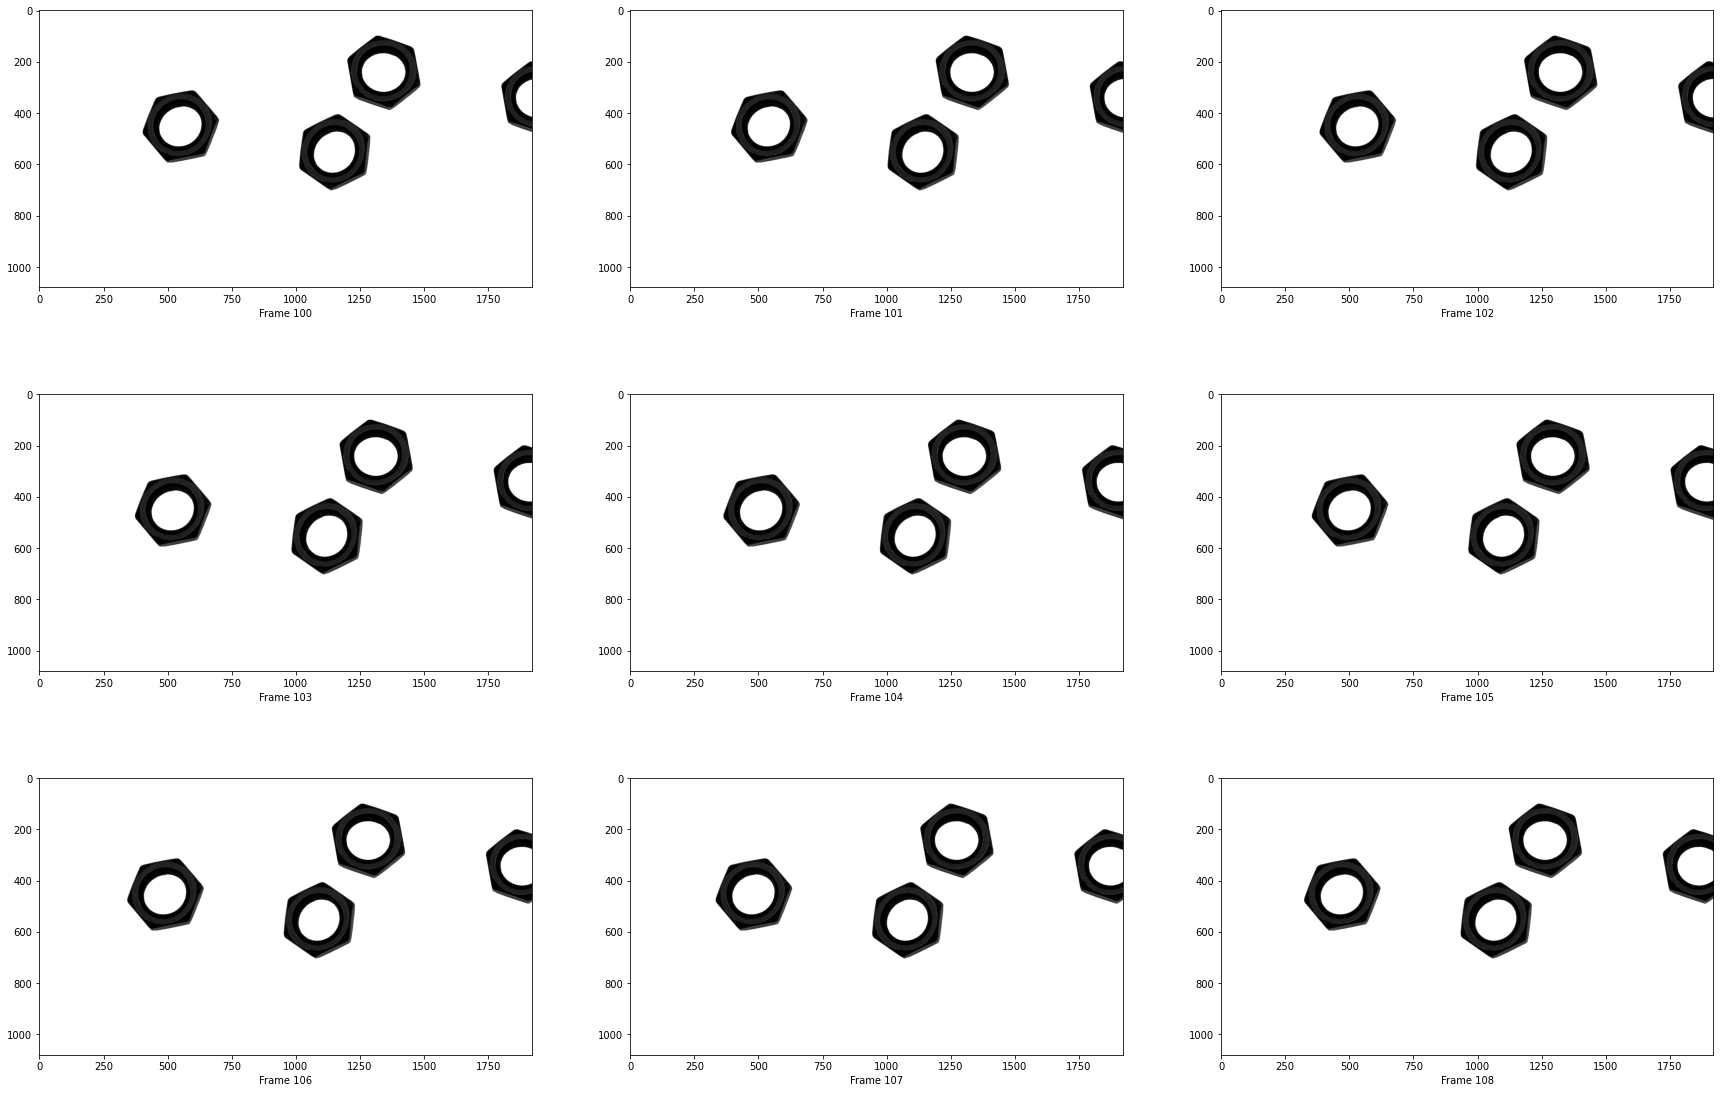
\includegraphics[scale=0.3]{figures/output_35_0.png}
    \end{figure}
    { \hspace*{\fill} \\}

\subsection{Finding contours of all connected components in a given frame}
    \begin{tcolorbox}[breakable, size=fbox, boxrule=1pt, pad at break*=1mm,colback=cellbackground, colframe=cellborder]
\prompt{In}{incolor}{20}{\boxspacing}
\begin{Verbatim}[commandchars=\\\{\}]
\PY{c+c1}{\PYZsh{} Find contours of all nuts present in a given frame of the belt}
\PY{n}{contour\PYZus{}plots} \PY{o}{=} \PY{p}{[}\PY{p}{]}
\PY{n}{contours\PYZus{}list} \PY{o}{=} \PY{p}{[}\PY{p}{]}
\PY{k}{for} \PY{n}{gray} \PY{o+ow}{in} \PY{n}{gray\PYZus{}frames}\PY{p}{:}
    \PY{c+c1}{\PYZsh{} finding contours}
    \PY{n}{\PYZus{}}\PY{p}{,} \PY{n}{labels}\PY{p}{,} \PY{n}{\PYZus{}}\PY{p}{,} \PY{n}{\PYZus{}} \PY{o}{=} \PY{n}{get\PYZus{}indexed\PYZus{}image}\PY{p}{(}\PY{n}{gray}\PY{p}{)} \PY{c+c1}{\PYZsh{} Conn: Comp: Analysis}
    \PY{n}{belt} \PY{o}{=} \PY{p}{(}\PY{p}{(}\PY{n}{labels} \PY{o}{\PYZgt{}}\PY{o}{=} \PY{l+m+mi}{1}\PY{p}{)}\PY{o}{*}\PY{l+m+mi}{255}\PY{p}{)}\PY{o}{.}\PY{n}{astype}\PY{p}{(}\PY{l+s+s1}{\PYZsq{}}\PY{l+s+s1}{uint8}\PY{l+s+s1}{\PYZsq{}}\PY{p}{)}
    \PY{n}{contours}\PY{p}{,}\PY{n}{\PYZus{}}  \PY{o}{=} \PY{n}{cv}\PY{o}{.}\PY{n}{findContours}\PY{p}{(}\PY{n}{belt}\PY{p}{,} \PY{n}{cv}\PY{o}{.}\PY{n}{RETR\PYZus{}EXTERNAL}\PY{p}{,} \PY{n}{cv}\PY{o}{.}\PY{n}{CHAIN\PYZus{}APPROX\PYZus{}SIMPLE}\PY{p}{)}
    \PY{n}{contours\PYZus{}list}\PY{o}{.}\PY{n}{append}\PY{p}{(}\PY{n}{contours}\PY{p}{)}
    \PY{c+c1}{\PYZsh{} plotting contours}
    \PY{n}{im\PYZus{}contours\PYZus{}belt} \PY{o}{=} \PY{n}{np}\PY{o}{.}\PY{n}{zeros}\PY{p}{(}\PY{p}{(}\PY{n}{belt}\PY{o}{.}\PY{n}{shape}\PY{p}{[}\PY{l+m+mi}{0}\PY{p}{]}\PY{p}{,}\PY{n}{belt}\PY{o}{.}\PY{n}{shape}\PY{p}{[}\PY{l+m+mi}{1}\PY{p}{]}\PY{p}{,}\PY{l+m+mi}{3}\PY{p}{)}\PY{p}{,} \PY{n}{np}\PY{o}{.}\PY{n}{uint8}\PY{p}{)}
    \PY{n}{cont\PYZus{}plot} \PY{o}{=} \PY{n}{cv}\PY{o}{.}\PY{n}{drawContours}\PY{p}{(}\PY{n}{im\PYZus{}contours\PYZus{}belt}\PY{p}{,} \PY{n}{contours}\PY{p}{,} \PY{o}{\PYZhy{}}\PY{l+m+mi}{1}\PY{p}{,} \PY{p}{(}\PY{l+m+mi}{0}\PY{p}{,}\PY{l+m+mi}{255}\PY{p}{,}\PY{l+m+mi}{0}\PY{p}{)}\PY{p}{,} \PY{l+m+mi}{5}\PY{p}{)}\PY{o}{.}\PY{n}{astype}\PY{p}{(}\PY{l+s+s1}{\PYZsq{}}\PY{l+s+s1}{uint8}\PY{l+s+s1}{\PYZsq{}}\PY{p}{)}
    \PY{n}{contour\PYZus{}plots}\PY{o}{.}\PY{n}{append}\PY{p}{(}\PY{n}{cont\PYZus{}plot}\PY{p}{)}
\end{Verbatim}
\end{tcolorbox}

    \begin{tcolorbox}[breakable, size=fbox, boxrule=1pt, pad at break*=1mm,colback=cellbackground, colframe=cellborder]
\prompt{In}{incolor}{21}{\boxspacing}
\begin{Verbatim}[commandchars=\\\{\}]
\PY{c+c1}{\PYZsh{} visualizing some of the contour plots on frames}
\PY{n}{plt}\PY{o}{.}\PY{n}{figure}\PY{p}{(}\PY{n}{figsize}\PY{o}{=}\PY{p}{(}\PY{l+m+mi}{30}\PY{p}{,}\PY{l+m+mi}{20}\PY{p}{)}\PY{p}{)}
\PY{k}{for} \PY{n}{i} \PY{o+ow}{in} \PY{n+nb}{range}\PY{p}{(}\PY{l+m+mi}{9}\PY{p}{)}\PY{p}{:}
    \PY{n}{plt}\PY{o}{.}\PY{n}{subplot}\PY{p}{(}\PY{l+m+mi}{3}\PY{p}{,}\PY{l+m+mi}{3}\PY{p}{,}\PY{n}{i}\PY{o}{+}\PY{l+m+mi}{1}\PY{p}{)}
    \PY{n}{plt}\PY{o}{.}\PY{n}{imshow}\PY{p}{(}\PY{n}{contour\PYZus{}plots}\PY{p}{[}\PY{l+m+mi}{100} \PY{o}{+}\PY{n}{i}\PY{p}{]}\PY{p}{)}
    \PY{n}{plt}\PY{o}{.}\PY{n}{xlabel}\PY{p}{(}\PY{l+s+s2}{\PYZdq{}}\PY{l+s+s2}{Frame }\PY{l+s+s2}{\PYZdq{}} \PY{o}{+} \PY{n+nb}{str}\PY{p}{(}\PY{l+m+mi}{100} \PY{o}{+}\PY{n}{i}\PY{p}{)}\PY{p}{)}
\PY{n}{plt}\PY{o}{.}\PY{n}{show}\PY{p}{(}\PY{p}{)}
\end{Verbatim}
\end{tcolorbox}

    \begin{figure}[!h]
		\centering
    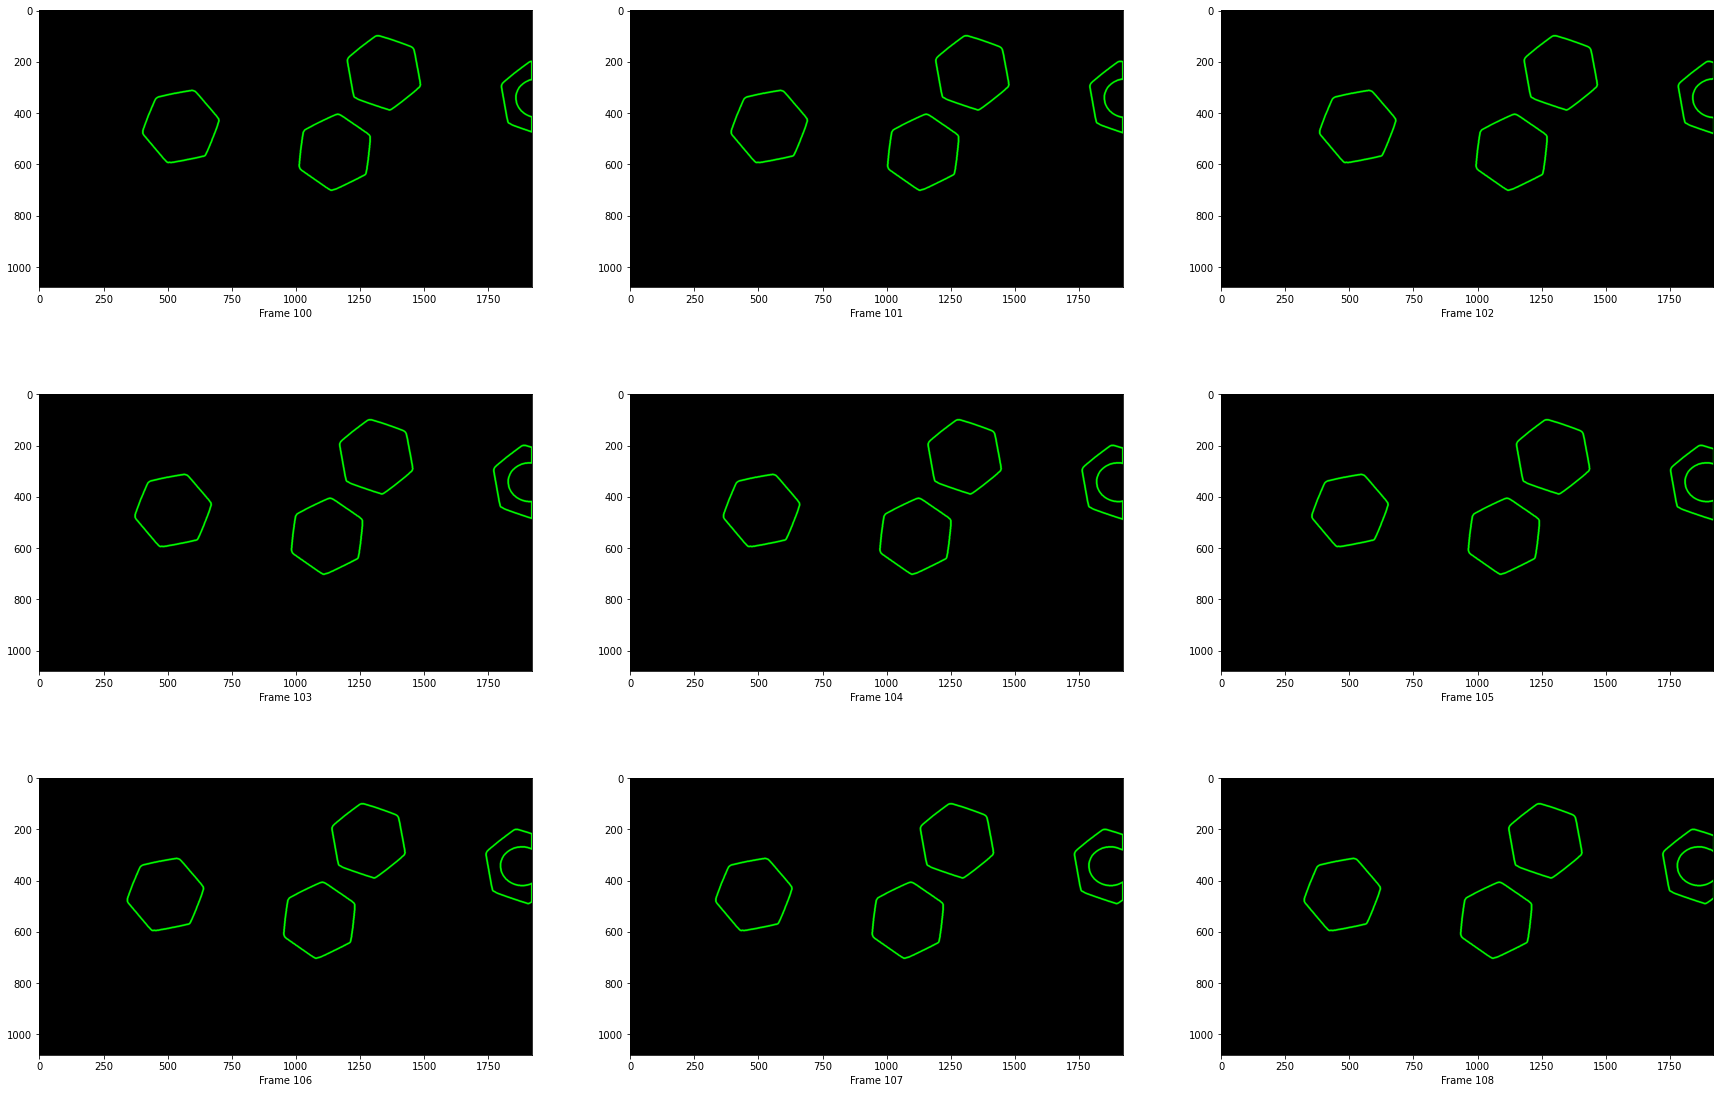
\includegraphics[scale=0.3]{figures/output_37_0.png}
    \end{figure}
    { \hspace*{\fill} \\}
\pagebreak
    \hypertarget{object-detection-and-tracking}{%
\section{Object detection and
tracking}\label{object-detection-and-tracking}}

For each contour of the belt frame,

\begin{enumerate}
\def\labelenumi{\arabic{enumi}.}
\tightlist
\item
  Use \texttt{is\_new} and \texttt{prev\_index} functions to track each
  frame and get the indices of each nut.
\item
  Write a code to detect and track hexagonal nuts in each frame.
\end{enumerate}

\textbf{Hint}: \emph{If you are thresholding on areas (template and
contour) you can use 500 as the threshold. You can set the matching
threshold to be 0.5 and experiment}.
\subsection{Extracting details about each contour in each frame}
    \begin{tcolorbox}[breakable, size=fbox, boxrule=1pt, pad at break*=1mm,colback=cellbackground, colframe=cellborder]
\prompt{In}{incolor}{22}{\boxspacing}
\begin{Verbatim}[commandchars=\\\{\}]
\PY{c+c1}{\PYZsh{} frame tracking through image moments}
\PY{c+c1}{\PYZsh{} extracting details about each contour in each frame}
\PY{n}{video} \PY{o}{=} \PY{p}{[}\PY{p}{]}
\PY{n+nb}{print}\PY{p}{(}\PY{l+s+s2}{\PYZdq{}}\PY{l+s+s2}{Details extraction is in progress...}\PY{l+s+s2}{\PYZdq{}}\PY{p}{)}
\PY{k}{for} \PY{n}{gray} \PY{o+ow}{in} \PY{n}{gray\PYZus{}frames}\PY{p}{:}
    \PY{c+c1}{\PYZsh{} finding contours}
    \PY{n}{\PYZus{}}\PY{p}{,} \PY{n}{labels}\PY{p}{,} \PY{n}{\PYZus{}}\PY{p}{,} \PY{n}{\PYZus{}} \PY{o}{=} \PY{n}{get\PYZus{}indexed\PYZus{}image}\PY{p}{(}\PY{n}{gray}\PY{p}{)}
    \PY{n}{belt} \PY{o}{=} \PY{p}{(}\PY{p}{(}\PY{n}{labels} \PY{o}{\PYZgt{}}\PY{o}{=} \PY{l+m+mi}{1}\PY{p}{)}\PY{o}{*}\PY{l+m+mi}{255}\PY{p}{)}\PY{o}{.}\PY{n}{astype}\PY{p}{(}\PY{l+s+s1}{\PYZsq{}}\PY{l+s+s1}{uint8}\PY{l+s+s1}{\PYZsq{}}\PY{p}{)}
    \PY{n}{contours}\PY{p}{,}\PY{n}{\PYZus{}}  \PY{o}{=} \PY{n}{cv}\PY{o}{.}\PY{n}{findContours}\PY{p}{(}\PY{n}{belt}\PY{p}{,} \PY{n}{cv}\PY{o}{.}\PY{n}{RETR\PYZus{}EXTERNAL}\PY{p}{,} \PY{n}{cv}\PY{o}{.}\PY{n}{CHAIN\PYZus{}APPROX\PYZus{}SIMPLE}\PY{p}{)}

    \PY{n}{count} \PY{o}{=} \PY{l+m+mi}{0} \PY{c+c1}{\PYZsh{} number of nuts in a given frame}
    \PY{n}{frame} \PY{o}{=} \PY{p}{[}\PY{p}{]}

    \PY{k}{for} \PY{n}{contour} \PY{o+ow}{in} \PY{n}{contours}\PY{p}{:}
        \PY{n}{metric} \PY{o}{=} \PY{n}{cv}\PY{o}{.}\PY{n}{matchShapes}\PY{p}{(}\PY{n}{contours\PYZus{}t}\PY{p}{[}\PY{l+m+mi}{0}\PY{p}{]}\PY{p}{,} \PY{n}{contour}\PY{p}{,} \PY{n}{cv}\PY{o}{.}\PY{n}{CONTOURS\PYZus{}MATCH\PYZus{}I1}\PY{p}{,} \PY{l+m+mf}{0.0}\PY{p}{)}
        \PY{c+c1}{\PYZsh{} Set the matching threshold to be 0.5}
        \PY{k}{if} \PY{n}{metric} \PY{o}{\PYZlt{}}\PY{o}{=} \PY{l+m+mf}{0.5}\PY{p}{:} \PY{c+c1}{\PYZsh{} if only a complete hexagonal nut}
            \PY{n}{count} \PY{o}{+}\PY{o}{=}\PY{l+m+mi}{1}
            \PY{n}{M}  \PY{o}{=} \PY{n}{cv}\PY{o}{.}\PY{n}{moments}\PY{p}{(}\PY{n}{contour}\PY{p}{)}
            \PY{n}{ca} \PY{o}{=} \PY{n}{M}\PY{p}{[}\PY{l+s+s1}{\PYZsq{}}\PY{l+s+s1}{m00}\PY{l+s+s1}{\PYZsq{}}\PY{p}{]}
            \PY{n}{cx}\PY{p}{,} \PY{n}{cy} \PY{o}{=} \PY{n+nb}{int}\PY{p}{(}\PY{n}{M}\PY{p}{[}\PY{l+s+s1}{\PYZsq{}}\PY{l+s+s1}{m10}\PY{l+s+s1}{\PYZsq{}}\PY{p}{]}\PY{o}{/}\PY{n}{M}\PY{p}{[}\PY{l+s+s1}{\PYZsq{}}\PY{l+s+s1}{m00}\PY{l+s+s1}{\PYZsq{}}\PY{p}{]}\PY{p}{)}\PY{p}{,} \PY{n+nb}{int}\PY{p}{(}\PY{n}{M}\PY{p}{[}\PY{l+s+s1}{\PYZsq{}}\PY{l+s+s1}{m01}\PY{l+s+s1}{\PYZsq{}}\PY{p}{]}\PY{o}{/}\PY{n}{M}\PY{p}{[}\PY{l+s+s1}{\PYZsq{}}\PY{l+s+s1}{m00}\PY{l+s+s1}{\PYZsq{}}\PY{p}{]}\PY{p}{)}
            \PY{n}{frame}\PY{o}{.}\PY{n}{append}\PY{p}{(}\PY{n}{np}\PY{o}{.}\PY{n}{array}\PY{p}{(}\PY{p}{[}\PY{n}{cx}\PY{p}{,} \PY{n}{cy}\PY{p}{,} \PY{n}{ca}\PY{p}{,} \PY{n}{count}\PY{p}{]}\PY{p}{)}\PY{p}{)}

    \PY{n}{video}\PY{o}{.}\PY{n}{append}\PY{p}{(}\PY{n}{frame}\PY{p}{)}
\PY{n+nb}{print}\PY{p}{(}\PY{l+s+s2}{\PYZdq{}}\PY{l+s+s2}{Details extraction completed.}\PY{l+s+s2}{\PYZdq{}}\PY{p}{)}
\end{Verbatim}
\end{tcolorbox}

    \begin{Verbatim}[commandchars=\\\{\}]
Details extraction is in progress{\ldots}
Details extraction completed.
    \end{Verbatim}
\pagebreak
\subsection{Nut counter Implementation}
    \begin{tcolorbox}[breakable, size=fbox, boxrule=1pt, pad at break*=1mm,colback=cellbackground, colframe=cellborder]
\prompt{In}{incolor}{23}{\boxspacing}
\begin{Verbatim}[commandchars=\\\{\}]
\PY{c+c1}{\PYZsh{} Nut counter Implementation}
\PY{c+c1}{\PYZsh{} last element keeps the number of nuts in a given frame. }
\PY{c+c1}{\PYZsh{} Therefore, initial number of nuts is as follows.}
\PY{n}{total\PYZus{}nuts} \PY{o}{=} \PY{n+nb}{int}\PY{p}{(}\PY{n}{video}\PY{p}{[}\PY{l+m+mi}{0}\PY{p}{]}\PY{p}{[}\PY{o}{\PYZhy{}}\PY{l+m+mi}{1}\PY{p}{]}\PY{p}{[}\PY{o}{\PYZhy{}}\PY{l+m+mi}{1}\PY{p}{]}\PY{p}{)}
\PY{n+nb}{print}\PY{p}{(}\PY{l+s+s2}{\PYZdq{}}\PY{l+s+s2}{Number of nuts in the zeroth frame: }\PY{l+s+s2}{\PYZdq{}}\PY{p}{,}\PY{n}{total\PYZus{}nuts}\PY{p}{)}

\PY{n}{delta\PYZus{}x} \PY{o}{=} \PY{n}{np}\PY{o}{.}\PY{n}{array}\PY{p}{(}\PY{p}{[}\PY{l+m+mi}{15}\PY{p}{]}\PY{p}{)}
\PY{n}{i} \PY{o}{=} \PY{n}{np}\PY{o}{.}\PY{n}{array}\PY{p}{(}\PY{p}{[}\PY{l+m+mi}{0}\PY{p}{]}\PY{p}{)}

\PY{n}{prev\PYZus{}frame} \PY{o}{=} \PY{n}{video}\PY{p}{[}\PY{l+m+mi}{0}\PY{p}{]} \PY{c+c1}{\PYZsh{} Reference frame to compare with the upcoming frame}

\PY{k}{for} \PY{n}{frame\PYZus{}num} \PY{o+ow}{in} \PY{n+nb}{range}\PY{p}{(}\PY{l+m+mi}{1}\PY{p}{,} \PY{n+nb}{len}\PY{p}{(}\PY{n}{video}\PY{p}{)}\PY{p}{)}\PY{p}{:}
    \PY{n}{current\PYZus{}frame} \PY{o}{=} \PY{n}{video}\PY{p}{[}\PY{n}{frame\PYZus{}num}\PY{p}{]} \PY{c+c1}{\PYZsh{} frame to be compared    }

    \PY{k}{for} \PY{n}{nut} \PY{o+ow}{in} \PY{n}{current\PYZus{}frame}\PY{p}{:}
        \PY{c+c1}{\PYZsh{} Checking the current nut with previous frame}
        \PY{c+c1}{\PYZsh{} if it is a new nut count it.}
        \PY{k}{if} \PY{n}{is\PYZus{}new}\PY{p}{(}\PY{n}{prev\PYZus{}frame}\PY{p}{,} \PY{n}{nut}\PY{p}{,} \PY{n}{delta\PYZus{}x}\PY{p}{,} \PY{n}{i}\PY{p}{)}\PY{p}{:}
            \PY{n}{total\PYZus{}nuts} \PY{o}{+}\PY{o}{=}\PY{l+m+mi}{1}

    \PY{n}{prev\PYZus{}frame} \PY{o}{=} \PY{n}{current\PYZus{}frame}

\PY{n+nb}{print}\PY{p}{(}\PY{l+s+s2}{\PYZdq{}}\PY{l+s+s2}{Total number of nuts found: }\PY{l+s+s2}{\PYZdq{}}\PY{p}{,}\PY{n}{total\PYZus{}nuts}\PY{p}{)}
\end{Verbatim}
\end{tcolorbox}

    \begin{Verbatim}[commandchars=\\\{\}]
Number of nuts in the zeroth frame:  1
Total number of nuts found:  5
    \end{Verbatim}
\subsection{Tracking nuts: An extension of the previous nut counting algorithm}
    \begin{tcolorbox}[breakable, size=fbox, boxrule=1pt, pad at break*=1mm,colback=cellbackground, colframe=cellborder]
\prompt{In}{incolor}{24}{\boxspacing}
\begin{Verbatim}[commandchars=\\\{\}]
\PY{c+c1}{\PYZsh{} trackig nuts: An extension of the previous counting nuts algorithm}
\PY{n+nb}{print}\PY{p}{(}\PY{l+s+s2}{\PYZdq{}}\PY{l+s+s2}{Detection and indexing is in progress...}\PY{l+s+s2}{\PYZdq{}}\PY{p}{)}
\PY{n}{total\PYZus{}nuts} \PY{o}{=} \PY{n+nb}{int}\PY{p}{(}\PY{n}{video}\PY{p}{[}\PY{l+m+mi}{0}\PY{p}{]}\PY{p}{[}\PY{o}{\PYZhy{}}\PY{l+m+mi}{1}\PY{p}{]}\PY{p}{[}\PY{o}{\PYZhy{}}\PY{l+m+mi}{1}\PY{p}{]}\PY{p}{)} \PY{c+c1}{\PYZsh{}initial number of nuts in frame 0}
\PY{n}{delta\PYZus{}x} \PY{o}{=} \PY{n}{np}\PY{o}{.}\PY{n}{array}\PY{p}{(}\PY{p}{[}\PY{l+m+mi}{15}\PY{p}{]}\PY{p}{)}
\PY{n}{i} \PY{o}{=} \PY{n}{np}\PY{o}{.}\PY{n}{array}\PY{p}{(}\PY{p}{[}\PY{l+m+mi}{0}\PY{p}{]}\PY{p}{)}
\PY{n}{prev\PYZus{}frame} \PY{o}{=} \PY{n}{video}\PY{p}{[}\PY{l+m+mi}{0}\PY{p}{]} \PY{c+c1}{\PYZsh{} Reference frame to compare with the upcoming frame}

\PY{k}{for} \PY{n}{frame\PYZus{}num} \PY{o+ow}{in} \PY{n+nb}{range}\PY{p}{(}\PY{l+m+mi}{1}\PY{p}{,} \PY{n+nb}{len}\PY{p}{(}\PY{n}{video}\PY{p}{)}\PY{p}{)}\PY{p}{:}
    \PY{n}{current\PYZus{}frame} \PY{o}{=} \PY{n}{video}\PY{p}{[}\PY{n}{frame\PYZus{}num}\PY{p}{]} \PY{c+c1}{\PYZsh{} frame to be compared}

    \PY{k}{for} \PY{n}{nut} \PY{o+ow}{in} \PY{n}{current\PYZus{}frame}\PY{p}{:}
        \PY{c+c1}{\PYZsh{} Checking the current nut with previous frame}
        \PY{c+c1}{\PYZsh{} if it is a new nut count it and assign a new index}
        \PY{k}{if} \PY{n}{is\PYZus{}new}\PY{p}{(}\PY{n}{prev\PYZus{}frame}\PY{p}{,} \PY{n}{nut}\PY{p}{,} \PY{n}{delta\PYZus{}x}\PY{p}{,} \PY{n}{i}\PY{p}{)}\PY{p}{:}
            \PY{n}{total\PYZus{}nuts} \PY{o}{+}\PY{o}{=}\PY{l+m+mi}{1}
            \PY{n}{nut}\PY{p}{[}\PY{o}{\PYZhy{}}\PY{l+m+mi}{1}\PY{p}{]} \PY{o}{=} \PY{n}{total\PYZus{}nuts} \PY{c+c1}{\PYZsh{} assignment of a new index}

        \PY{k}{else}\PY{p}{:}
            \PY{c+c1}{\PYZsh{} to be tracked the nut must not be a new nut}
            \PY{n}{nut\PYZus{}index} \PY{o}{=} \PY{n}{prev\PYZus{}index}\PY{p}{(}\PY{n}{prev\PYZus{}frame}\PY{p}{,} \PY{n}{nut}\PY{p}{,} \PY{n}{delta\PYZus{}x}\PY{p}{,} \PY{n}{i}\PY{p}{)}
            \PY{n}{nut}\PY{p}{[}\PY{o}{\PYZhy{}}\PY{l+m+mi}{1}\PY{p}{]} \PY{o}{=} \PY{n}{nut\PYZus{}index} \PY{c+c1}{\PYZsh{} assign the same index it had previously, for old nuts}

    \PY{n}{prev\PYZus{}frame} \PY{o}{=} \PY{n}{current\PYZus{}frame}
\PY{n+nb}{print}\PY{p}{(}\PY{l+s+s2}{\PYZdq{}}\PY{l+s+s2}{Detection and indexing completed.}\PY{l+s+s2}{\PYZdq{}}\PY{p}{)}
\end{Verbatim}
\end{tcolorbox}

    \begin{Verbatim}[commandchars=\\\{\}]
Detection and indexing is in progress{\ldots}
Detection and indexing completed.
    \end{Verbatim}
\subsection{Frame annotation with the extracted details}
    \begin{tcolorbox}[breakable, size=fbox, boxrule=1pt, pad at break*=1mm,colback=cellbackground, colframe=cellborder]
\prompt{In}{incolor}{25}{\boxspacing}
\begin{Verbatim}[commandchars=\\\{\}]
\PY{c+c1}{\PYZsh{} frame annotation with the extracted details}

\PY{n}{annotated\PYZus{}frames} \PY{o}{=}\PY{p}{[}\PY{p}{]}
\PY{n}{frame\PYZus{}num} \PY{o}{=} \PY{l+m+mi}{0}
\PY{n+nb}{print}\PY{p}{(}\PY{l+s+s2}{\PYZdq{}}\PY{l+s+s2}{Frame annotation is in progress...}\PY{l+s+s2}{\PYZdq{}}\PY{p}{)}
\PY{k}{for} \PY{n}{frame}\PY{p}{,} \PY{n}{color\PYZus{}frame}\PY{p}{,} \PY{n}{contours} \PY{o+ow}{in} \PY{n+nb}{zip}\PY{p}{(}\PY{n}{video}\PY{p}{,} \PY{n}{color\PYZus{}frames}\PY{p}{,} \PY{n}{contours\PYZus{}list}\PY{p}{)}\PY{p}{:}

    \PY{c+c1}{\PYZsh{} Annotation was done on the frames of the original video}
    \PY{n}{img} \PY{o}{=} \PY{n}{color\PYZus{}frame}
    \PY{n}{y} \PY{o}{=} \PY{l+m+mi}{0} \PY{c+c1}{\PYZsh{} to change the vertical position of \PYZsq{}object details\PYZsq{} of a frame}

    \PY{k}{for} \PY{n}{nut} \PY{o+ow}{in} \PY{n}{frame}\PY{p}{:}
        \PY{c+c1}{\PYZsh{} Annotate the nut index}
        \PY{n}{img} \PY{o}{=} \PY{n}{cv}\PY{o}{.}\PY{n}{putText}\PY{p}{(}\PY{n}{img}\PY{p}{,} \PY{n+nb}{str}\PY{p}{(}\PY{n+nb}{int}\PY{p}{(}\PY{n}{nut}\PY{p}{[}\PY{o}{\PYZhy{}}\PY{l+m+mi}{1}\PY{p}{]}\PY{p}{)}\PY{p}{)}\PY{p}{,}\PYZbs{}
                \PY{p}{(}\PY{n+nb}{int}\PY{p}{(}\PY{n}{nut}\PY{p}{[}\PY{l+m+mi}{0}\PY{p}{]}\PY{p}{)}\PY{p}{,}\PY{n+nb}{int}\PY{p}{(}\PY{n}{nut}\PY{p}{[}\PY{l+m+mi}{1}\PY{p}{]}\PY{p}{)}\PY{p}{)}\PY{p}{,}\PY{n}{cv}\PY{o}{.}\PY{n}{FONT\PYZus{}HERSHEY\PYZus{}SIMPLEX}\PY{p}{,} \PY{l+m+mi}{2}\PY{p}{,} \PY{p}{(}\PY{l+m+mi}{255}\PY{p}{,}\PY{l+m+mi}{0}\PY{p}{,}\PY{l+m+mi}{0}\PY{p}{)}\PY{p}{,} \PY{l+m+mi}{4}\PY{p}{)}
        \PY{c+c1}{\PYZsh{} Annotate the nut(object) details}
        \PY{n}{img} \PY{o}{=} \PY{n}{cv}\PY{o}{.}\PY{n}{putText}\PY{p}{(}\PY{n}{img}\PY{p}{,} \PY{l+s+s2}{\PYZdq{}}\PY{l+s+s2}{Object }\PY{l+s+si}{\PYZob{}\PYZcb{}}\PY{l+s+s2}{: }\PY{l+s+si}{\PYZob{}:04\PYZcb{}}\PY{l+s+s2}{ }\PY{l+s+si}{\PYZob{}:04\PYZcb{}}\PY{l+s+s2}{ }\PY{l+s+si}{\PYZob{}:05\PYZcb{}}\PY{l+s+s2}{\PYZdq{}}\PY{o}{.}\PY{n}{format}\PY{p}{(}\PY{n+nb}{int}\PY{p}{(}\PY{n}{nut}\PY{p}{[}\PY{o}{\PYZhy{}}\PY{l+m+mi}{1}\PY{p}{]}\PY{p}{)}\PY{p}{,} \PY{n+nb}{int}\PY{p}{(}\PY{n}{nut}\PY{p}{[}\PY{l+m+mi}{0}\PY{p}{]}\PY{p}{)}\PY{p}{,} \PY{n+nb}{int}\PY{p}{(}\PY{n}{nut}\PY{p}{[}\PY{l+m+mi}{1}\PY{p}{]}\PY{p}{)}\PY{p}{,} \PY{n}{nut}\PY{p}{[}\PY{l+m+mi}{2}\PY{p}{]}\PY{p}{)}\PY{p}{,}\PYZbs{}
                         \PY{p}{(}\PY{l+m+mi}{50}\PY{p}{,}\PY{l+m+mi}{850} \PY{o}{+} \PY{l+m+mi}{70}\PY{o}{*}\PY{n}{y}\PY{p}{)}\PY{p}{,} \PY{n}{cv}\PY{o}{.}\PY{n}{FONT\PYZus{}HERSHEY\PYZus{}SIMPLEX}\PY{p}{,} \PY{l+m+mi}{2}\PY{p}{,} \PY{p}{(}\PY{l+m+mi}{255}\PY{p}{,}\PY{l+m+mi}{0}\PY{p}{,}\PY{l+m+mi}{0}\PY{p}{)}\PY{p}{,} \PY{l+m+mi}{4}\PY{p}{)}

        \PY{n}{y} \PY{o}{+}\PY{o}{=}\PY{l+m+mi}{1} \PY{c+c1}{\PYZsh{} change vertical position for next object details annotation.}

    \PY{c+c1}{\PYZsh{} Annotation of the frame number and draw the extracted contours}
    \PY{n}{img} \PY{o}{=} \PY{n}{cv}\PY{o}{.}\PY{n}{putText}\PY{p}{(}\PY{n}{img}\PY{p}{,} \PY{l+s+s2}{\PYZdq{}}\PY{l+s+s2}{Frame }\PY{l+s+s2}{\PYZdq{}}\PY{o}{+}\PY{n+nb}{str}\PY{p}{(}\PY{n}{frame\PYZus{}num}\PY{p}{)} \PY{p}{,} \PY{p}{(}\PY{l+m+mi}{50}\PY{p}{,}\PY{l+m+mi}{750}\PY{p}{)} \PY{p}{,} \PY{n}{cv}\PY{o}{.}\PY{n}{FONT\PYZus{}HERSHEY\PYZus{}SIMPLEX}\PY{p}{,} \PY{l+m+mi}{2}\PY{p}{,} \PY{p}{(}\PY{l+m+mi}{255}\PY{p}{,}\PY{l+m+mi}{0}\PY{p}{,}\PY{l+m+mi}{0}\PY{p}{)}\PY{p}{,} \PY{l+m+mi}{3}\PY{p}{)}
    \PY{n}{img} \PY{o}{=} \PY{n}{cv}\PY{o}{.}\PY{n}{drawContours}\PY{p}{(}\PY{n}{img}\PY{p}{,} \PY{n}{contours}\PY{p}{,} \PY{o}{\PYZhy{}}\PY{l+m+mi}{1}\PY{p}{,} \PY{p}{(}\PY{l+m+mi}{255}\PY{p}{,}\PY{l+m+mi}{0}\PY{p}{,}\PY{l+m+mi}{0}\PY{p}{)}\PY{p}{,} \PY{l+m+mi}{5}\PY{p}{)}\PY{o}{.}\PY{n}{astype}\PY{p}{(}\PY{l+s+s1}{\PYZsq{}}\PY{l+s+s1}{uint8}\PY{l+s+s1}{\PYZsq{}}\PY{p}{)}

    \PY{c+c1}{\PYZsh{} Index number 180631J}
    \PY{n}{img} \PY{o}{=} \PY{n}{cv}\PY{o}{.}\PY{n}{putText}\PY{p}{(}\PY{n}{img}\PY{p}{,} \PY{l+s+s2}{\PYZdq{}}\PY{l+s+s2}{180631J}\PY{l+s+s2}{\PYZdq{}} \PY{p}{,} \PY{p}{(}\PY{l+m+mi}{50}\PY{p}{,}\PY{l+m+mi}{150}\PY{p}{)} \PY{p}{,} \PY{n}{cv}\PY{o}{.}\PY{n}{FONT\PYZus{}HERSHEY\PYZus{}SIMPLEX}\PY{p}{,} \PY{l+m+mi}{2}\PY{p}{,} \PY{p}{(}\PY{l+m+mi}{255}\PY{p}{,}\PY{l+m+mi}{0}\PY{p}{,}\PY{l+m+mi}{0}\PY{p}{)}\PY{p}{,} \PY{l+m+mi}{3}\PY{p}{)}
    \PY{n}{annotated\PYZus{}frames}\PY{o}{.}\PY{n}{append}\PY{p}{(}\PY{n}{img}\PY{p}{)}
    \PY{n}{frame\PYZus{}num} \PY{o}{+}\PY{o}{=}\PY{l+m+mi}{1}
\PY{n+nb}{print}\PY{p}{(}\PY{l+s+s2}{\PYZdq{}}\PY{l+s+s2}{Frame annotation completed.}\PY{l+s+s2}{\PYZdq{}}\PY{p}{)}
\end{Verbatim}
\end{tcolorbox}

    \begin{Verbatim}[commandchars=\\\{\}]
Frame annotation is in progress{\ldots}
Frame annotation completed.
    \end{Verbatim}

    \begin{tcolorbox}[breakable, size=fbox, boxrule=1pt, pad at break*=1mm,colback=cellbackground, colframe=cellborder]
\prompt{In}{incolor}{26}{\boxspacing}
\begin{Verbatim}[commandchars=\\\{\}]
\PY{c+c1}{\PYZsh{} visulaizing some annotated frames }
\PY{n}{plt}\PY{o}{.}\PY{n}{figure}\PY{p}{(}\PY{n}{figsize}\PY{o}{=}\PY{p}{(}\PY{l+m+mi}{30}\PY{p}{,}\PY{l+m+mi}{20}\PY{p}{)}\PY{p}{)}
\PY{k}{for} \PY{n}{i} \PY{o+ow}{in} \PY{n+nb}{range}\PY{p}{(}\PY{l+m+mi}{9}\PY{p}{)}\PY{p}{:}
    \PY{n}{plt}\PY{o}{.}\PY{n}{subplot}\PY{p}{(}\PY{l+m+mi}{3}\PY{p}{,}\PY{l+m+mi}{3}\PY{p}{,}\PY{n}{i}\PY{o}{+}\PY{l+m+mi}{1}\PY{p}{)}
    \PY{n}{plt}\PY{o}{.}\PY{n}{imshow}\PY{p}{(}\PY{n}{annotated\PYZus{}frames}\PY{p}{[}\PY{l+m+mi}{100} \PY{o}{+}\PY{n}{i}\PY{p}{]}\PY{p}{[}\PY{p}{:}\PY{p}{,}\PY{p}{:}\PY{p}{,}\PY{p}{:}\PY{p}{:}\PY{o}{\PYZhy{}}\PY{l+m+mi}{1}\PY{p}{]}\PY{p}{)}
    \PY{n}{plt}\PY{o}{.}\PY{n}{xlabel}\PY{p}{(}\PY{l+s+s2}{\PYZdq{}}\PY{l+s+s2}{Frame }\PY{l+s+s2}{\PYZdq{}} \PY{o}{+} \PY{n+nb}{str}\PY{p}{(}\PY{l+m+mi}{100} \PY{o}{+}\PY{n}{i}\PY{p}{)}\PY{p}{)}
\PY{n}{plt}\PY{o}{.}\PY{n}{show}\PY{p}{(}\PY{p}{)}
\end{Verbatim}
\end{tcolorbox}

    \begin{figure}[!h]
		\centering
    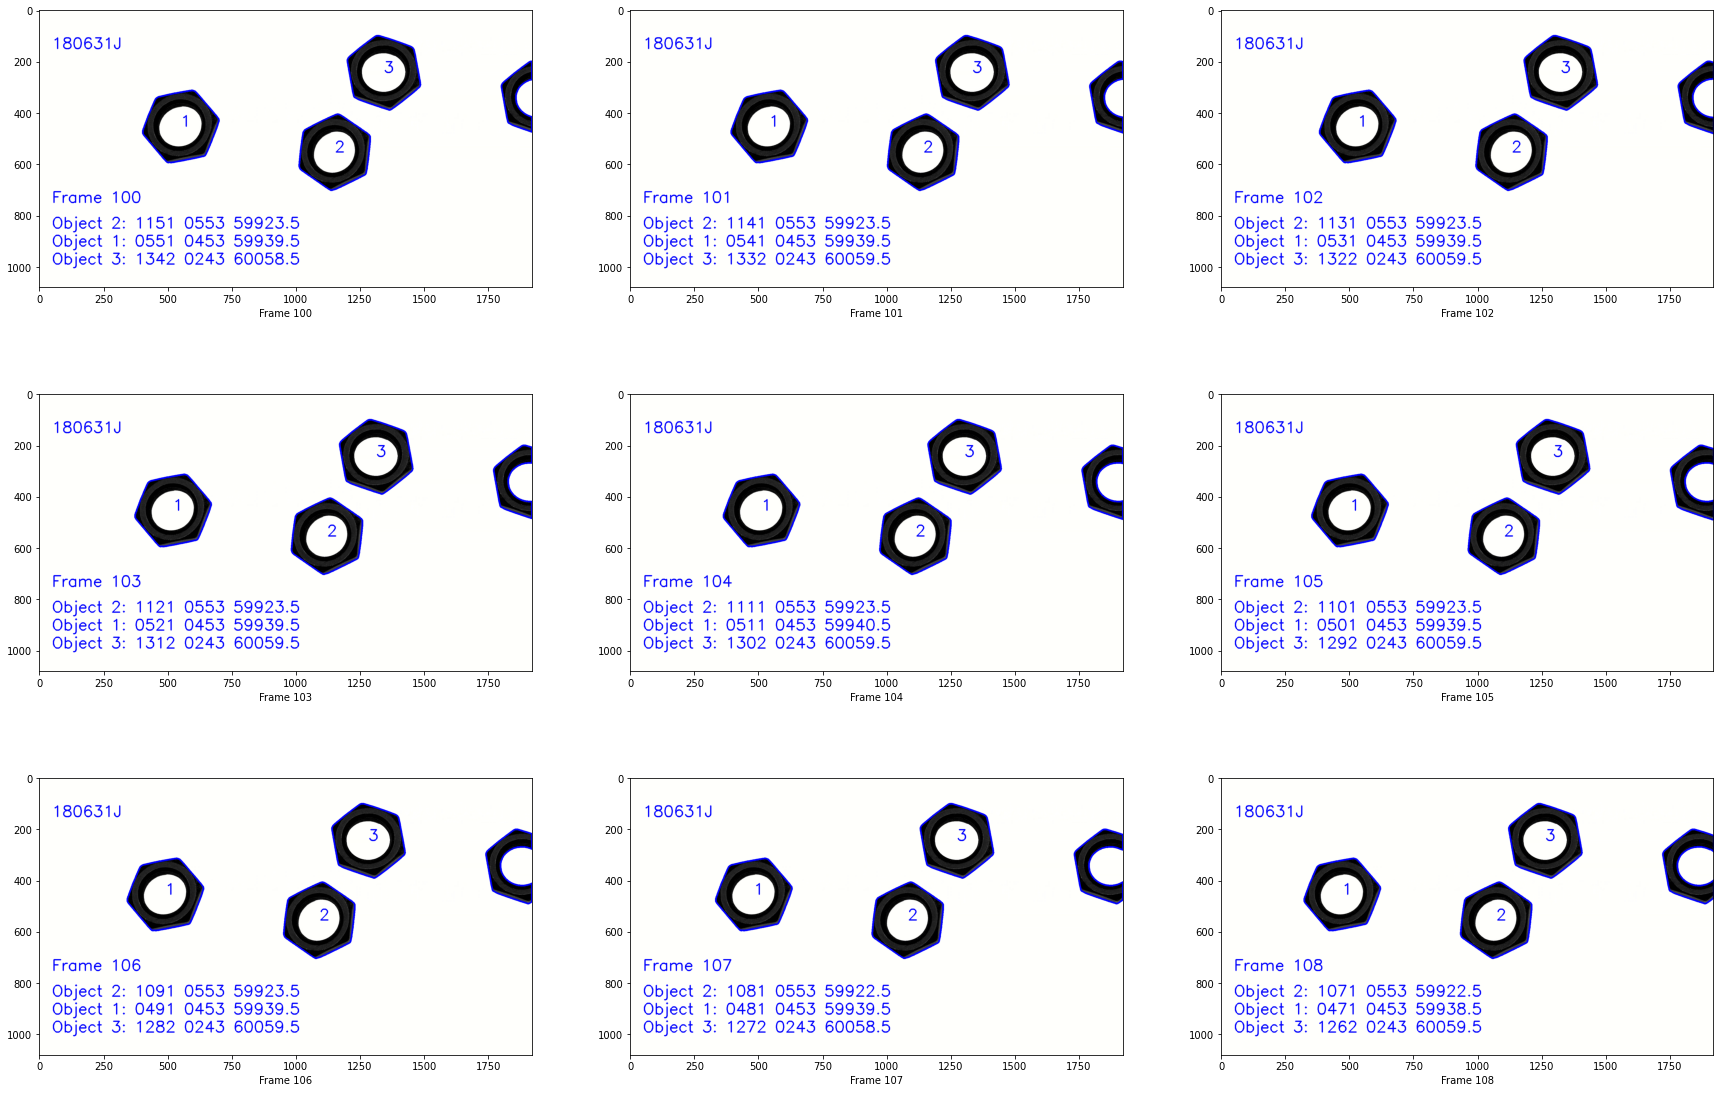
\includegraphics[scale=0.3]{figures/output_43_0.png}
    \end{figure}
    { \hspace*{\fill} \\}
\pagebreak
    \hypertarget{save-the-frames-as-a-video}{%
\subsection{Save the frames as a
video}\label{save-the-frames-as-a-video}}

    \begin{tcolorbox}[breakable, size=fbox, boxrule=1pt, pad at break*=1mm,colback=cellbackground, colframe=cellborder]
\prompt{In}{incolor}{27}{\boxspacing}
\begin{Verbatim}[commandchars=\\\{\}]
\PY{c+c1}{\PYZsh{} Defining necessary parameters for video write}

\PY{n}{output} \PY{o}{=} \PY{l+s+s1}{\PYZsq{}}\PY{l+s+s1}{180631j\PYZus{}en2550\PYZus{}a05.mp4}\PY{l+s+s1}{\PYZsq{}} \PY{c+c1}{\PYZsh{} Name of the output video file.}
\PY{n}{fourcc} \PY{o}{=} \PY{n}{cv}\PY{o}{.}\PY{n}{VideoWriter\PYZus{}fourcc}\PY{p}{(}\PY{o}{*}\PY{l+s+s1}{\PYZsq{}}\PY{l+s+s1}{MP4V}\PY{l+s+s1}{\PYZsq{}}\PY{p}{)} \PY{c+c1}{\PYZsh{} 4\PYZhy{}character code of codec used to compress the frames}
\PY{n}{duration} \PY{o}{=} \PY{l+m+mi}{9} \PY{c+c1}{\PYZsh{} duration of the source video}
\PY{n}{fps} \PY{o}{=} \PY{n+nb}{int}\PY{p}{(}\PY{n+nb}{len}\PY{p}{(}\PY{n}{annotated\PYZus{}frames}\PY{p}{)}\PY{o}{/}\PY{n}{duration}\PY{p}{)} \PY{c+c1}{\PYZsh{} Framerate of the created video stream}
\PY{n}{height}\PY{p}{,} \PY{n}{width}\PY{p}{,}\PY{n}{\PYZus{}} \PY{o}{=} \PY{n}{annotated\PYZus{}frames}\PY{p}{[}\PY{l+m+mi}{0}\PY{p}{]}\PY{o}{.}\PY{n}{shape}
\PY{n}{frame\PYZus{}size} \PY{o}{=} \PY{p}{(}\PY{n}{width}\PY{p}{,} \PY{n}{height}\PY{p}{)}
\PY{n}{isColor} \PY{o}{=} \PY{k+kc}{True} \PY{c+c1}{\PYZsh{} to write color images to the video}
\PY{n+nb}{print}\PY{p}{(}\PY{l+s+s1}{\PYZsq{}}\PY{l+s+s1}{Frame Size(WxH) :}\PY{l+s+s1}{\PYZsq{}}\PY{p}{,} \PY{n}{frame\PYZus{}size} \PY{p}{,}\PY{l+s+s1}{\PYZsq{}}\PY{l+s+se}{\PYZbs{}n}\PY{l+s+s1}{Frames Per Second :}\PY{l+s+s1}{\PYZsq{}}\PY{p}{,} \PY{n}{fps}\PY{p}{)}

\PY{c+c1}{\PYZsh{} Creating the Video Writer object}
\PY{n}{out} \PY{o}{=} \PY{n}{cv}\PY{o}{.}\PY{n}{VideoWriter}\PY{p}{(}\PY{n}{output}\PY{p}{,} \PY{n}{fourcc}\PY{p}{,} \PY{n}{fps}\PY{p}{,} \PY{n}{frame\PYZus{}size}\PY{p}{,} \PY{n}{isColor}\PY{p}{)}
\PY{n+nb}{print}\PY{p}{(}\PY{l+s+s2}{\PYZdq{}}\PY{l+s+s2}{Video writer in progress...}\PY{l+s+s2}{\PYZdq{}}\PY{p}{)}
\PY{k}{for} \PY{n}{frame} \PY{o+ow}{in} \PY{n}{annotated\PYZus{}frames}\PY{p}{:}
    \PY{n}{out}\PY{o}{.}\PY{n}{write}\PY{p}{(}\PY{n}{frame}\PY{p}{)}

\PY{c+c1}{\PYZsh{} Release everything if job is finished}
\PY{n}{out}\PY{o}{.}\PY{n}{release}\PY{p}{(}\PY{p}{)}
\PY{n+nb}{print}\PY{p}{(}\PY{l+s+s2}{\PYZdq{}}\PY{l+s+s2}{Video writing completed.}\PY{l+s+s2}{\PYZdq{}}\PY{p}{)}
\end{Verbatim}
\end{tcolorbox}

    \begin{Verbatim}[commandchars=\\\{\}]
Frame Size(WxH) : (1920, 1080)
Frames Per Second : 31
Video writer in progress{\ldots}
Video writing completed.
    \end{Verbatim}

\vfill
    % Add a bibliography block to the postdoc
 \begin{center}
	\textit{ \textbf{-- Executable code can be found on}} \href{https://github.com/bimalka98/Computer-Vision-and-Image-Processing/blob/main/EN2550Assignments/A5/180631j_en2550_a05.ipynb}{\faGithub} \textbf{\textit{--}}
\end{center}


\end{document}
